\documentclass[11pt,a4paper]{article}

\usepackage[margin=2.4cm]{geometry}
\usepackage[T1]{fontenc}
\usepackage{lmodern}
\usepackage{graphicx}
\usepackage{booktabs}
\usepackage{amsmath}
\usepackage{siunitx}
\usepackage{float}
\usepackage[section]{placeins}
\usepackage{xcolor}
\usepackage[font=small,labelfont=bf]{caption}
\usepackage[round]{natbib}
\usepackage[hidelinks]{hyperref}

\graphicspath{{figures/}}
\sisetup{detect-weight=true, group-separator={,}}

\setlength{\parskip}{0.4em}
\setlength{\parindent}{0pt}

\title{\vspace{-1.2cm}\textbf{Structure over Length:\\
Benchmarking Vienna's Bicycle Network against a Synthetically Grown Optimum}\\[0.3em]
\large A single-city deep dive in a five-city European context}
\author{Arthur Wunder \,(12431488)\\ \small Interdisciplinary Project}
\date{2026}

\begin{document}
\maketitle
\vspace{-0.8em}

\begin{abstract}
\noindent
Vienna has expanded its bicycle network incrementally over decades, more in response to
budgets and street redesigns than to network-level planning. This report asks how the
\emph{existing} network compares structurally to a theoretically grown optimum, in terms
of connectivity, spatial reach and routing efficiency. Three networks are compared
throughout: the physically separated paths \textbf{A}, the full rideable network
\textbf{B}, and the synthetic optimum \textbf{C}. Each network is reduced to a metric
graph, and a small set of structural indicators together with a spatial overlap analysis
is computed with a reproducible Python pipeline. The picture is consistent: Vienna's
network is spatially excellent but under-connected. It reaches almost the whole city, yet
its routing is measurably less efficient than the optimum, and its safe, physically
separated layer is barely connected at all. A five-city comparison places Vienna mid-pack.
The central recommendation is to connect existing fragments and add a small number of
strategic links rather than to add raw kilometres.
\end{abstract}

\section{Introduction}

Vienna's cycle network has grown to roughly 1{,}660\,km of mixed infrastructure and is
still expanding \citep{wiencyclenet}. Much of that growth has been incremental, following
budgets and street redesigns rather than a single connectivity blueprint; only recently
has closing the gaps in the main network and building cross-district links become an
explicit, funded programme \citep{wienradprogramm}. Such piecemeal development is typical
of urban cycling networks, which tend to grow in a fragmented, unplanned way
\citep{szell2022}. The plausible consequence is a structural weakness that a coverage map
hides: isolated segments, missing cross-connections and unnecessary detours. Whether a
cycling network \emph{functions} depends less on its total length than on its topology, on
whether its pieces connect into routes people can actually ride.

\paragraph{Research question.} How does the existing Vienna bicycle network compare
structurally to a synthetically grown, algorithmically optimised network in terms of
\emph{coverage}, \emph{connectivity} and \emph{spatial logic}? This decomposes into four
sub-questions: (i) How fragmented is the real network? (ii) Where are the largest
structural gaps? (iii) Does the current network follow a discernible network logic, or
rather an opportunistic growth pattern? (iv) Which connections would yield the greatest
structural improvement?

The comparison is deliberately structural and spatial rather than a length-normalised
benchmark: the two networks differ in total length, and that difference is interpreted
rather than eliminated by matching. The contribution is therefore as much methodological
as empirical, providing a transparent, reproducible pipeline that turns raw geodata into
comparable structural indicators.

\section{Data and Methods}

The analysis follows the standard data-science arc: acquire and clean heterogeneous
geodata, model each network as a graph, compute a fixed set of structural and spatial
indicators, and compare. Each step is described below; all of it is scripted and
re-runnable.

\subsection{Data sources}

\paragraph{Vienna (deep dive).} The real Vienna network is the official City of Vienna OGD
cycling dataset \citep{viennaogd}: 14{,}777 segments with \texttt{WKT} (well-known-text)
geometries in geographic coordinates (EPSG:4326) and a categorical attribute
(\texttt{MERKMAL}) distinguishing infrastructure types. This is the authoritative source
for the focus city and is used for the entire single-city analysis (Sec.~\ref{sec:vienna}).

\paragraph{Five cities (context).} For Amsterdam, Barcelona, Berlin, Oslo and Vienna the
real networks are extracted from OpenStreetMap \citep{osm} via \texttt{OSMnx}
\citep{boeing2017}. Comparable official municipal datasets do not exist for the other four
cities, and the growth algorithm itself operates on OSM, so OSM is the only consistent
multi-city source.

\paragraph{Why two sources is not a flaw.} Using the better local source (OGD) for the
focus city and the only consistent source (OSM) for the comparison is a deliberate
trade-off that does not distort the conclusions. For Vienna the two sources yield almost
identical structural metrics: directness 0.690 against 0.697, global efficiency 0.557
against 0.549, and an LCC share of 89\,\% in both. Where they differ is total length, and
this is purely a matter of definition: the City's published headline is about 1{,}660\,km
of designated cycle network \citep{wiencyclenet}, the OGD rideable network analysed here
measures 1{,}810\,km, and the broader OSM ``bikeable'' definition reaches 2{,}856\,km
because it also admits calmed and low-speed streets. Each is a wider definition of ``where
one may cycle'' than the last. The structure that this report is about is therefore robust
to the data choice; only absolute lengths must not be compared across sources.

\subsection{Preprocessing and network construction}

Before any metric is computed, all geometry is reprojected from EPSG:4326 to
\textbf{EPSG:31256} (MGI Austria GK East) so that lengths, buffers and areas are measured
in metres, and invalid geometries are dropped.

\emph{From geometry to graph.} Each network is converted to an undirected graph
\(G=(V,E)\): every \texttt{LINESTRING} is split into its constituent segments, segment
endpoints are snapped to a 2\,m grid so that geometrically coincident endpoints become a
single node \(v\in V\), and each segment becomes a weighted edge carrying its metric
length. The OSM networks need one further step. \texttt{OSMnx} stores a two-way street as
two directed edges, each carrying the full length, which would double-count bidirectional
infrastructure by up to \(1.9\times\); edges are therefore collapsed to undirected form,
one edge per physical segment, so that the reported lengths match the canonical results
exactly.

\paragraph{What counts as each network (OSM tag criteria).} The two real OSM networks are
built from explicit OpenStreetMap tag filters, so the boundary between ``protected'' and
``merely ridable'' is precise and reproducible. Network~A (\emph{biketrack}), the protected
or physically separated layer, is the union of ways tagged \texttt{cycleway=track},
\texttt{highway=cycleway}, \texttt{highway=path} with \texttt{bicycle=designated},
\texttt{cycleway:left=track}, \texttt{cycleway:right=track}, \texttt{cyclestreet} and
\texttt{bicycle\_road}, together with cyclist crossings (\texttt{cycleway=crossing}) snapped
onto it within 8\,m as connectors. Network~B (\emph{bikeable}), every edge that may legally
and reasonably be cycled, extends A with two further classes: all drivable streets whose
speed limit is at most 30\,km/h (\texttt{maxspeed} of 5, 10, 15, 20 or 30\,km/h, or the mph
equivalents), and calmed streets tagged \texttt{highway=living\_street}. A is therefore a
strict subset of B: A is what is physically protected, while B additionally includes
low-speed mixed traffic. Network~C is the synthetic optimum and carries no OSM tags. (For
Vienna's deep dive the protected layer is taken instead from the OGD \texttt{MERKMAL}
attribute; see Sec.~\ref{sec:safe}.)

\subsection{The synthetic optimum: \texttt{bikenwgrowth}}

The synthetic benchmark is generated by \texttt{bikenwgrowth} \citep{szell2022}, which
grows a bicycle network on top of the existing street graph. Points of interest (POIs) are
sampled on a regular grid of spacing \texttt{gridl}, and the network is then grown in 40
stages by greedy triangulation, at each stage adding the connection that most improves
global structure. Edges are prioritised by their \emph{betweenness centrality}, the number
of shortest paths that pass through an edge, weighted by proximity to the grid-sampled
POIs. Betweenness rewards links that carry many routes, so the algorithm builds a
structurally efficient skeleton rather than a dense web. The trajectory is summarised by a
growth quantile \(Q\in[0,1]\), the fraction of total growth completed, and the synthetic
optimum \(C\) is defined as the final stage \(Q=1.0\).

The grid spacing is the key free parameter. The Vienna deep dive uses a fine
\texttt{gridl} = 600\,m grid, with denser POIs and a 989\,km optimum, to resolve local
structure, while the five-city comparison uses the coarser 1701\,m grid of
\citet{szell2022}, whose sparser POIs yield a leaner 626\,km skeleton, for cross-city
comparability. The same algorithm on the same street network therefore produces two
visibly different optima depending only on the grid (Fig.~\ref{fig:gridl}): a denser,
more capillary network at 600\,m and a leaner arterial one at 1701\,m. Vienna's synthetic
figures consequently differ slightly between the deep dive and the cross-city run, an
effect revisited in Sec.~\ref{sec:limits}.

\begin{figure}[tbp]
\centering
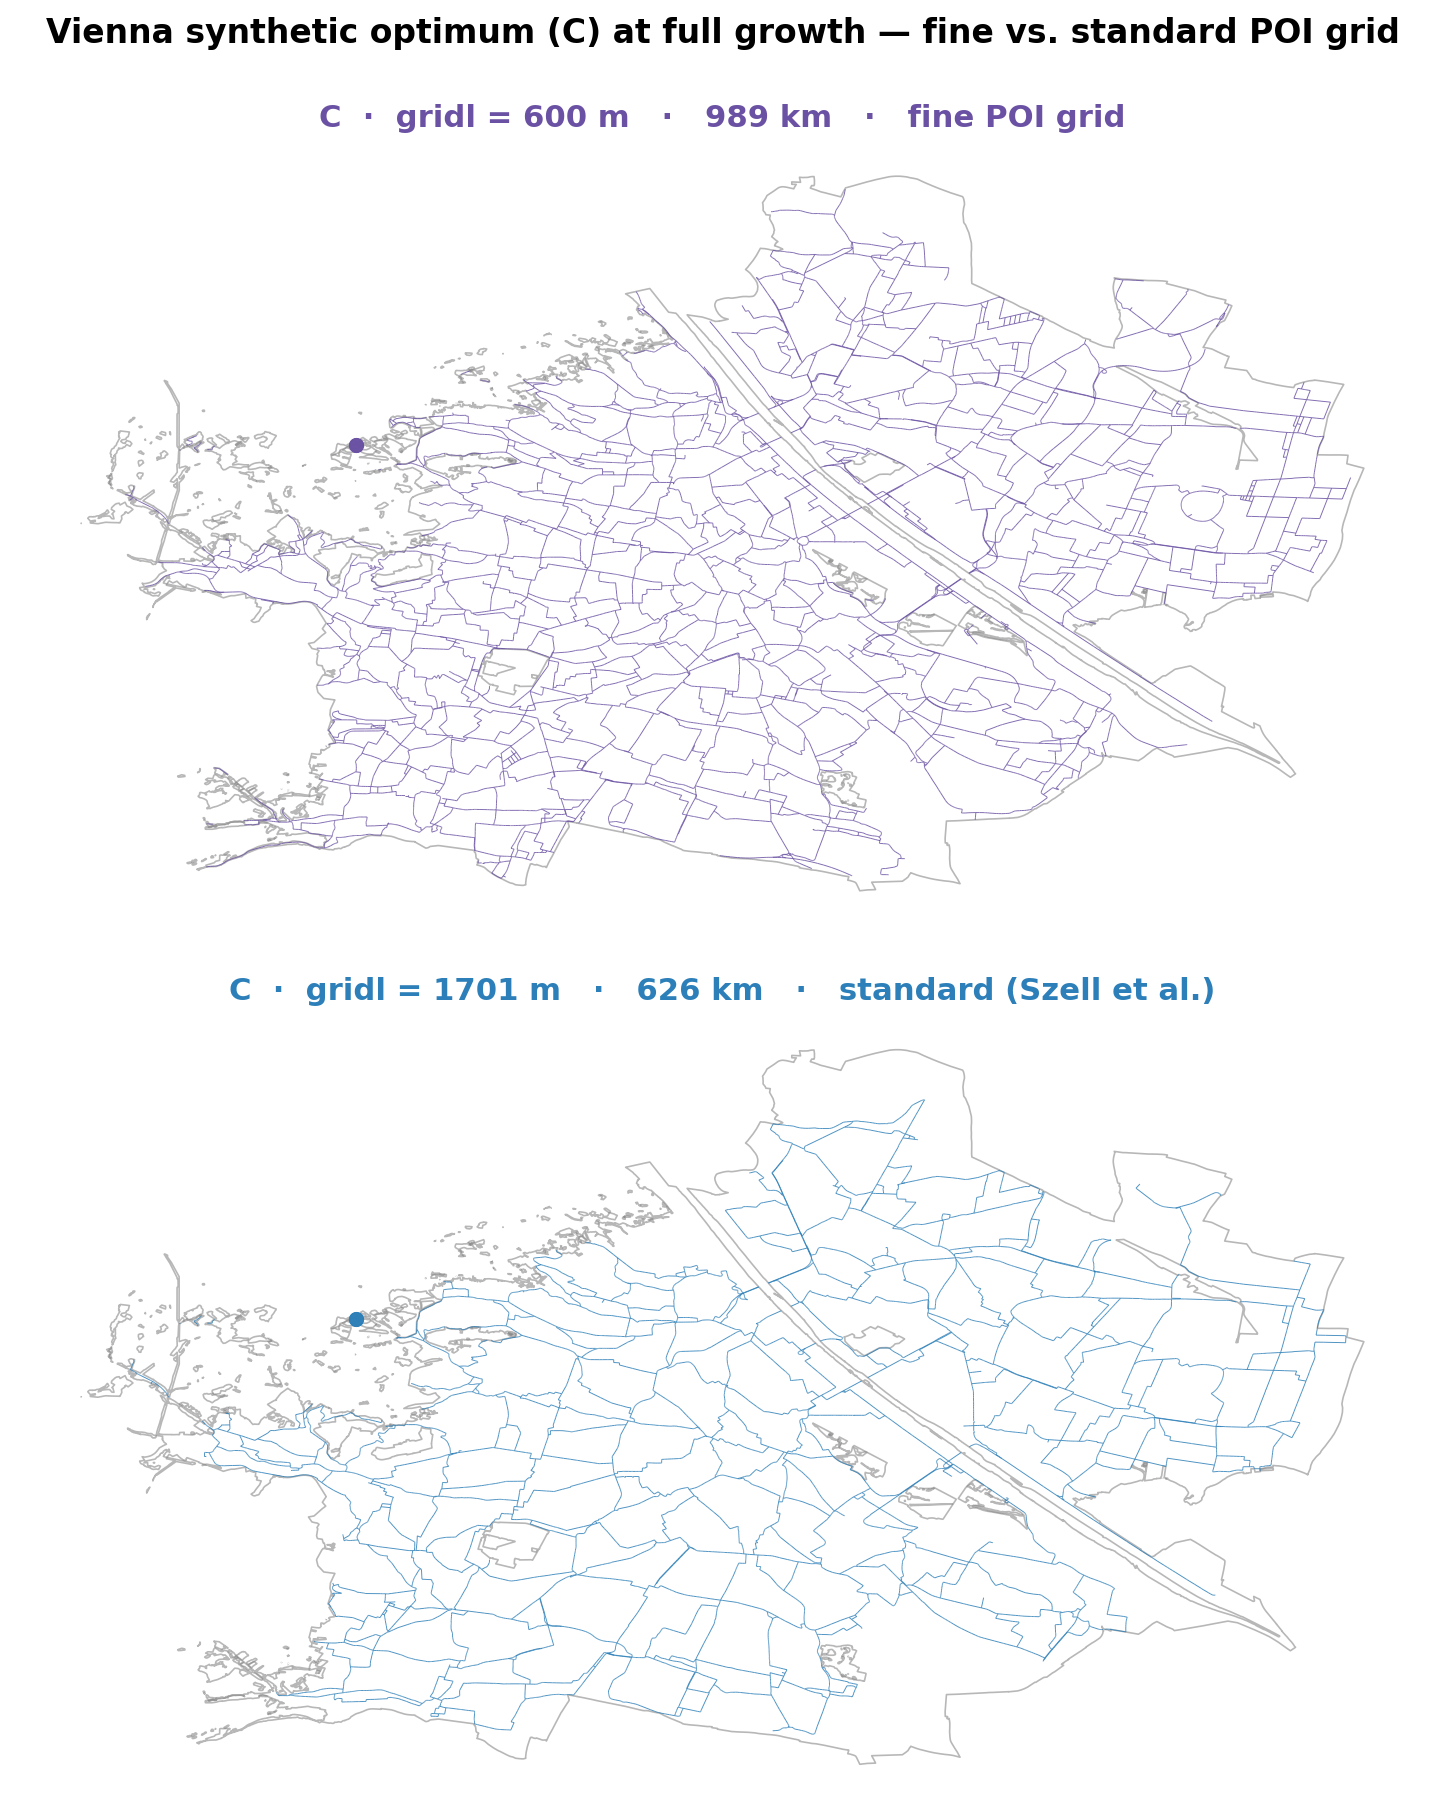
\includegraphics[width=0.62\linewidth]{vienna_gridl_networks.png}
\caption{Vienna's synthetic optimum \(C\) at full growth on a fine 600\,m POI grid (top,
989\,km) and on the standard 1701\,m grid (bottom, 626\,km), both clipped to the effective
boundary. The algorithm and street network are identical; the grid spacing alone decides
whether \(C\) becomes a dense, capillary network or a lean arterial skeleton, which is why
the synthetic optimum is a representative rather than a unique target.}
\label{fig:gridl}
\end{figure}

\subsection{Structural metrics}

Four indicators (Table~\ref{tab:metrics}) capture connectivity, routing quality and reach.
They are taken directly from the GrowBikeNet methodology of \citet{szell2022} and computed
with that project's own published code, the same \texttt{calculate\_*} routines used to grow
and score the synthetic optimum. Re-using the original definitions rather than
re-implementing them matters here: it guarantees that the real networks and \(C\) are
measured on exactly the same footing, so any difference between them is a property of the
networks and not of two different metric implementations. Let \(G\) have edge set \(E\) with
lengths \(\ell_e\); let the largest connected component (LCC) be \(G_{\mathrm{LCC}}\).

\emph{Component structure} is the number of connected components together with the
\emph{LCC share} \(L_{\mathrm{LCC}}/L_{\mathrm{tot}}\), the length in the largest component
over total length, where a value near 1 means the network is one reachable piece.
\emph{Directness} follows \citet{szell2022}: from a random sample of nodes in the LCC it
divides the total straight-line distance between connected pairs by the total network
distance,
\begin{equation}
\mathrm{Dir} = \frac{\sum_{(i,j)\in S} d_{\mathrm{euclid}}(i,j)}{\sum_{(i,j)\in S} d_{\mathrm{net}}(i,j)}\,,
\end{equation}
so \(\mathrm{Dir}=1\) means no detour and lower values mean more circuitous routes.
\emph{Global efficiency} \citep{latora2001} sums the inverse network distance over node
pairs and, following \citet{szell2022}, normalises it by the same sum for the ideal
straight-line network,
\begin{equation}
E_{\mathrm{glob}} = \frac{\sum_{i\neq j} 1/d_{\mathrm{net}}(i,j)}{\sum_{i\neq j} 1/d_{\mathrm{euclid}}(i,j)}\,,
\end{equation}
with disconnected pairs contributing \(0\) to the numerator. The normalisation places the
value on a \([0,1]\) scale, and because unreachable pairs count as zero it penalises
fragmentation directly, combining ``can I get there at all?'' and ``how directly?'' in one
number. Both directness and global efficiency are estimated over the pairs of a random sample of up
to 500 nodes (the GrowBikeNet default) rather than over all node pairs, which keeps the
computation tractable on large graphs at the cost of the small sampling variance noted in
Sec.~\ref{sec:limits}; a fixed random seed makes each run reproducible. \emph{Spatial
coverage} is the share of the city area within a 500\,m buffer of the
network, roughly a five-minute walk,
\(\mathrm{Cov}=\mathrm{Area}\!\big(\mathcal{B}_{500}(G)\cap\text{City}\big)/\mathrm{Area}(\text{City})\),
and answers ``can I reach a cycle path from here?''. The effective city area subtracts
large forest and park polygons so that uninhabited green space does not deflate coverage.

\begin{table}[t]
\centering
\caption{Structural and spatial metrics, what each captures, and how it is computed.}
\label{tab:metrics}
\small
\begin{tabular}{p{2.7cm}p{6.0cm}p{5.6cm}}
\toprule
Metric & Captures & Computation \\
\midrule
Components / LCC share & Fragmentation; how much of the network forms one reachable piece &
graph components; length in LCC \(/\) total length \\
Directness & Detour factor within the connected core &
\(\sum d_{\mathrm{euclid}} \big/ \sum d_{\mathrm{net}}\) over connected pairs (node sample, LCC) \\
Global efficiency & Connectivity and directness in one number; penalises islands &
\(\sum 1/d_{\mathrm{net}} \big/ \sum 1/d_{\mathrm{euclid}}\); disconnected \(=0\) \\
Spatial coverage & Reach: is the network nearby? &
area within 500\,m buffer \(/\) effective city area \\
Overlap / gap & How much of \(C\) already exists in the real network &
\(C\) edge is overlap if \(\ge 50\%\) of its 15\,m buffer lies within the real buffer \\
\bottomrule
\end{tabular}
\end{table}

\subsection{Spatial overlap and gap}

To ask \emph{which} of the optimum's connections already exist, each synthetic edge \(e\)
is buffered by 15\,m and classified as \emph{overlap} (already built) if at least half of
that buffer lies within 15\,m of the real network, and as \emph{gap} (missing) otherwise:
\begin{equation}
e \in \text{overlap} \iff
\frac{\mathrm{Area}\!\big(\mathcal{B}_{15}(e)\cap\mathcal{B}_{15}(R)\big)}
{\mathrm{Area}\!\big(\mathcal{B}_{15}(e)\big)} \ge 0.5 .
\end{equation}
Computing this naively, by intersecting every synthetic edge against the union of all real
buffers, is \(O(N^2)\) and intractable on dense networks. The real buffers are instead
indexed in an R-tree (\texttt{shapely.STRtree}), and each synthetic edge is tested only
against locally relevant candidates, which is exact but orders of magnitude faster.

\subsection{Implementation and reproducibility}

The full pipeline is Python: \texttt{pandas} and \texttt{numpy} for tabular data,
\texttt{geopandas} and \texttt{shapely} for geometric operations, and \texttt{networkx}
for graph metrics. Every figure and table in this report is produced from the same scripted
outputs, and the analysis is deterministic, using a fixed random seed for the directness
and efficiency sampling. It transfers to any city for which OSM or an equivalent local
dataset is available. All code, the data-processing pipeline and the source of this report
are openly available at \url{https://github.com/ACWunder/bike-szell}.

The results follow in two parts: a single-city deep dive into Vienna
(Sec.~\ref{sec:vienna}), then a five-city comparison that places it in an international
context (Sec.~\ref{sec:crosscity}).

\section{Vienna: a structural deep dive}
\label{sec:vienna}

This first part of the results examines Vienna on its own, taking the official OGD network
as the real reference and the fine 600\,m optimum as the benchmark. Table~\ref{tab:glance}
gives the headline comparison, and the subsections then take each dimension in turn, from
connectivity and routing quality to spatial coverage, the overlap between the real and the
optimal network, and finally the safe, physically separated layer on its own.

\begin{table}[t]
\centering
\caption{Vienna at a glance: full real network (B) against the synthetic optimum (C),
600\,m grid. Source: OGD analysis.}
\label{tab:glance}
\small
\begin{tabular}{lccc}
\toprule
Metric & \textbf{B} (real) & \textbf{C} (synthetic) & Gap \\
\midrule
Global efficiency      & 0.557  & 0.653  & \textcolor{red!70!black}{$-14.6\,\%$} \\
Directness (LCC)       & 0.690  & 0.745  & \textcolor{red!70!black}{$-7.4\,\%$} \\
LCC share              & 89.4\,\% & 100\,\% & \textcolor{red!70!black}{$-10.6$\,pp} \\
Spatial coverage       & 90.7\,\% & 89.3\,\% & \textcolor{green!45!black}{$+1.4$\,pp} \\
Overlap (C in B)       & 56.7\,\% & n/a & 43.3\,\% gap \\
Total length           & 1{,}810\,km & 989\,km & n/a \\
\bottomrule
\end{tabular}
\end{table}

\subsection{Connectivity}

Vienna's full rideable network (B) is 1{,}810\,km long and splits into 546 connected
components, yet it is functionally connected: 89.4\,\% of its length belongs to one giant
connected component. The 545 remaining components are small peripheral stubs, short
dead-ends and not-yet-joined fragments that together contribute only 11\,\% of the length.
The synthetic network is a single component by construction. At the level of the combined
network, then, connectivity is good. As Sec.~\ref{sec:safe} shows, however, this
connectivity is bought by mixing all infrastructure types together, and the safe layer
alone tells a very different story.

\subsection{Efficiency, directness and coverage}

Figure~\ref{fig:growth} plots the quality metrics along the synthetic growth and marks
Vienna's real network on the same axes, locating it relative to the optimum at every
length. Two readings follow. First, Vienna's global efficiency of 0.557 is 14.6\,\% below
the optimum's 0.653, and its directness of 0.690 is 7.4\,\% below 0.745. These gaps are
meaningful but bridgeable: the optimum reaches its higher efficiency with only about
989\,km, far less than Vienna's 1{,}810\,km. The deficit is therefore one of arrangement
rather than quantity, since a strategically built network of the same size would score
higher.

Second, the directness gap of 7.4\,\% is markedly smaller than the efficiency gap of
14.6\,\%. Directness is measured only within the connected core, whereas efficiency counts
disconnected pairs as zero, so the difference between the two gaps is precisely the
signature of fragmentation. Where Vienna's network connects, its routes are already quite
direct; the larger efficiency penalty comes from pairs that cannot be reached at all.

Coverage is the one metric where the real network wins: 90.7\,\% of Vienna's area lies
within 500\,m of the network, marginally above the optimum's 89.3\,\%. Vienna's
infrastructure is thus excellently distributed in space. The problem is not where it is,
but how it connects.

\begin{figure}[t]
\centering
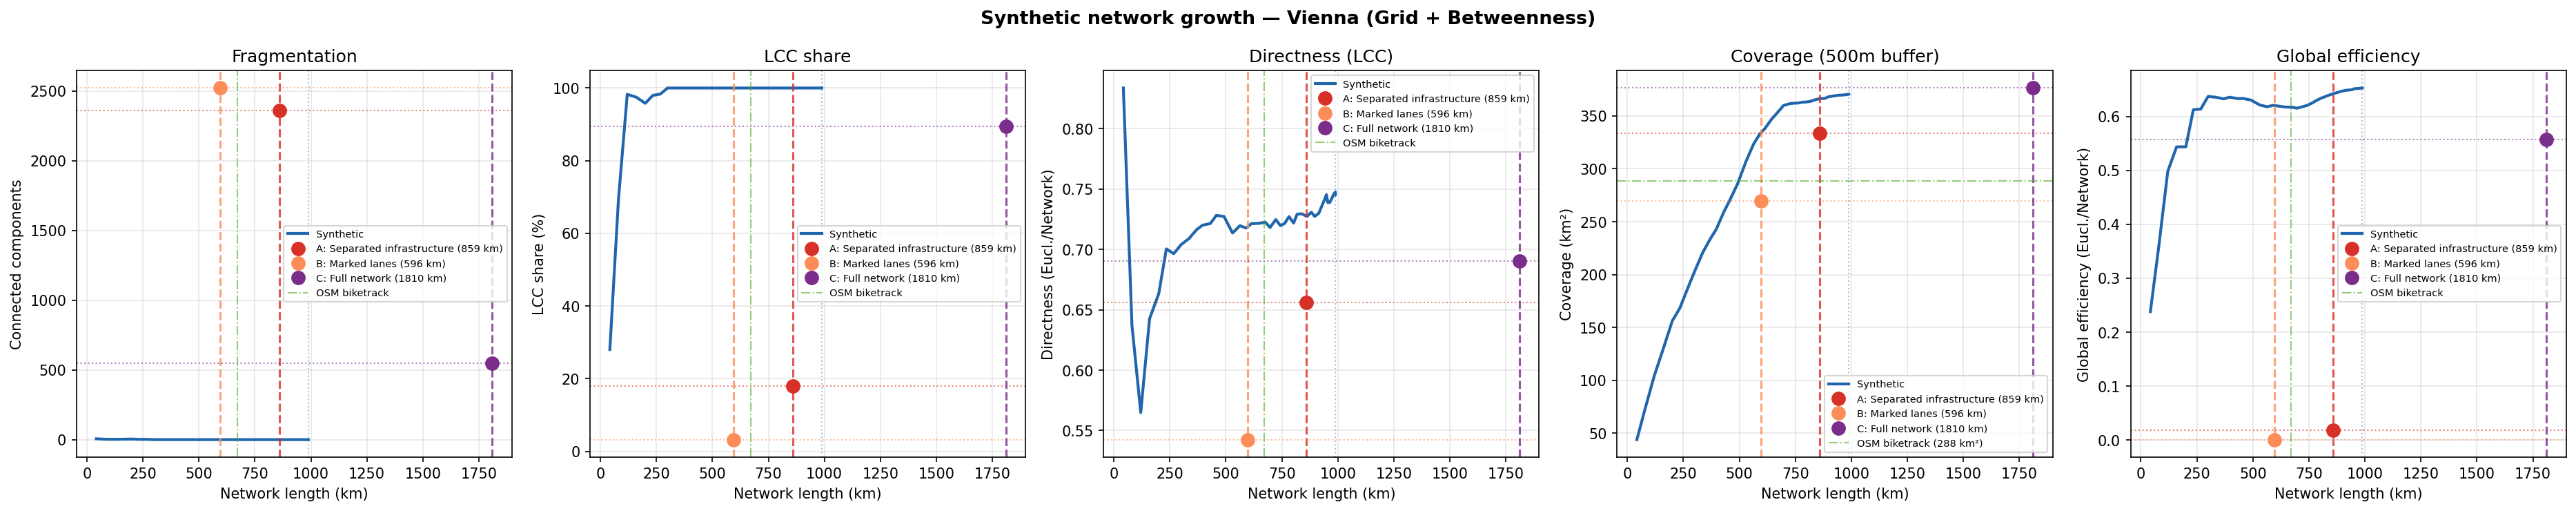
\includegraphics[width=0.98\linewidth]{vienna_growth.png}
\caption{Quality of the synthetic network along its growth, with network length on the
$x$-axis and Vienna's real network marked as points. Coverage saturates early, while global
efficiency keeps climbing as the optimum links its components, the gap Vienna has yet to
close.}
\label{fig:growth}
\end{figure}

\subsection{Spatial overlap and gap}
\label{sec:gap}

A spatial comparison of the optimum against the real network shows that 56.7\,\% of \(C\)
already exists in Vienna, an overlap of 561\,km, while the remaining 429\,km does not
(Fig.~\ref{fig:overlap}). The interpretation requires care, because the two networks are
deliberately of different size. The optimum is a lean, efficient skeleton of 989\,km rather
than a dense web, whereas the real network of 1{,}810\,km is denser overall and especially
so in the inner city, which already contains the skeleton. This is why the core of
Fig.~\ref{fig:overlap} is mostly overlap with little gap.

The 43\,\% gap is therefore not evidence that Vienna is ``too sparse''. It is the
comparatively few high-betweenness links the optimum would add, and they concentrate in the
outer districts rather than the well-covered centre. These are precisely the connections
with the highest structural value per kilometre, a spatially explicit list of where new
infrastructure would most improve the network. This answers sub-questions (ii) and (iv).

\begin{figure}[t]
\centering
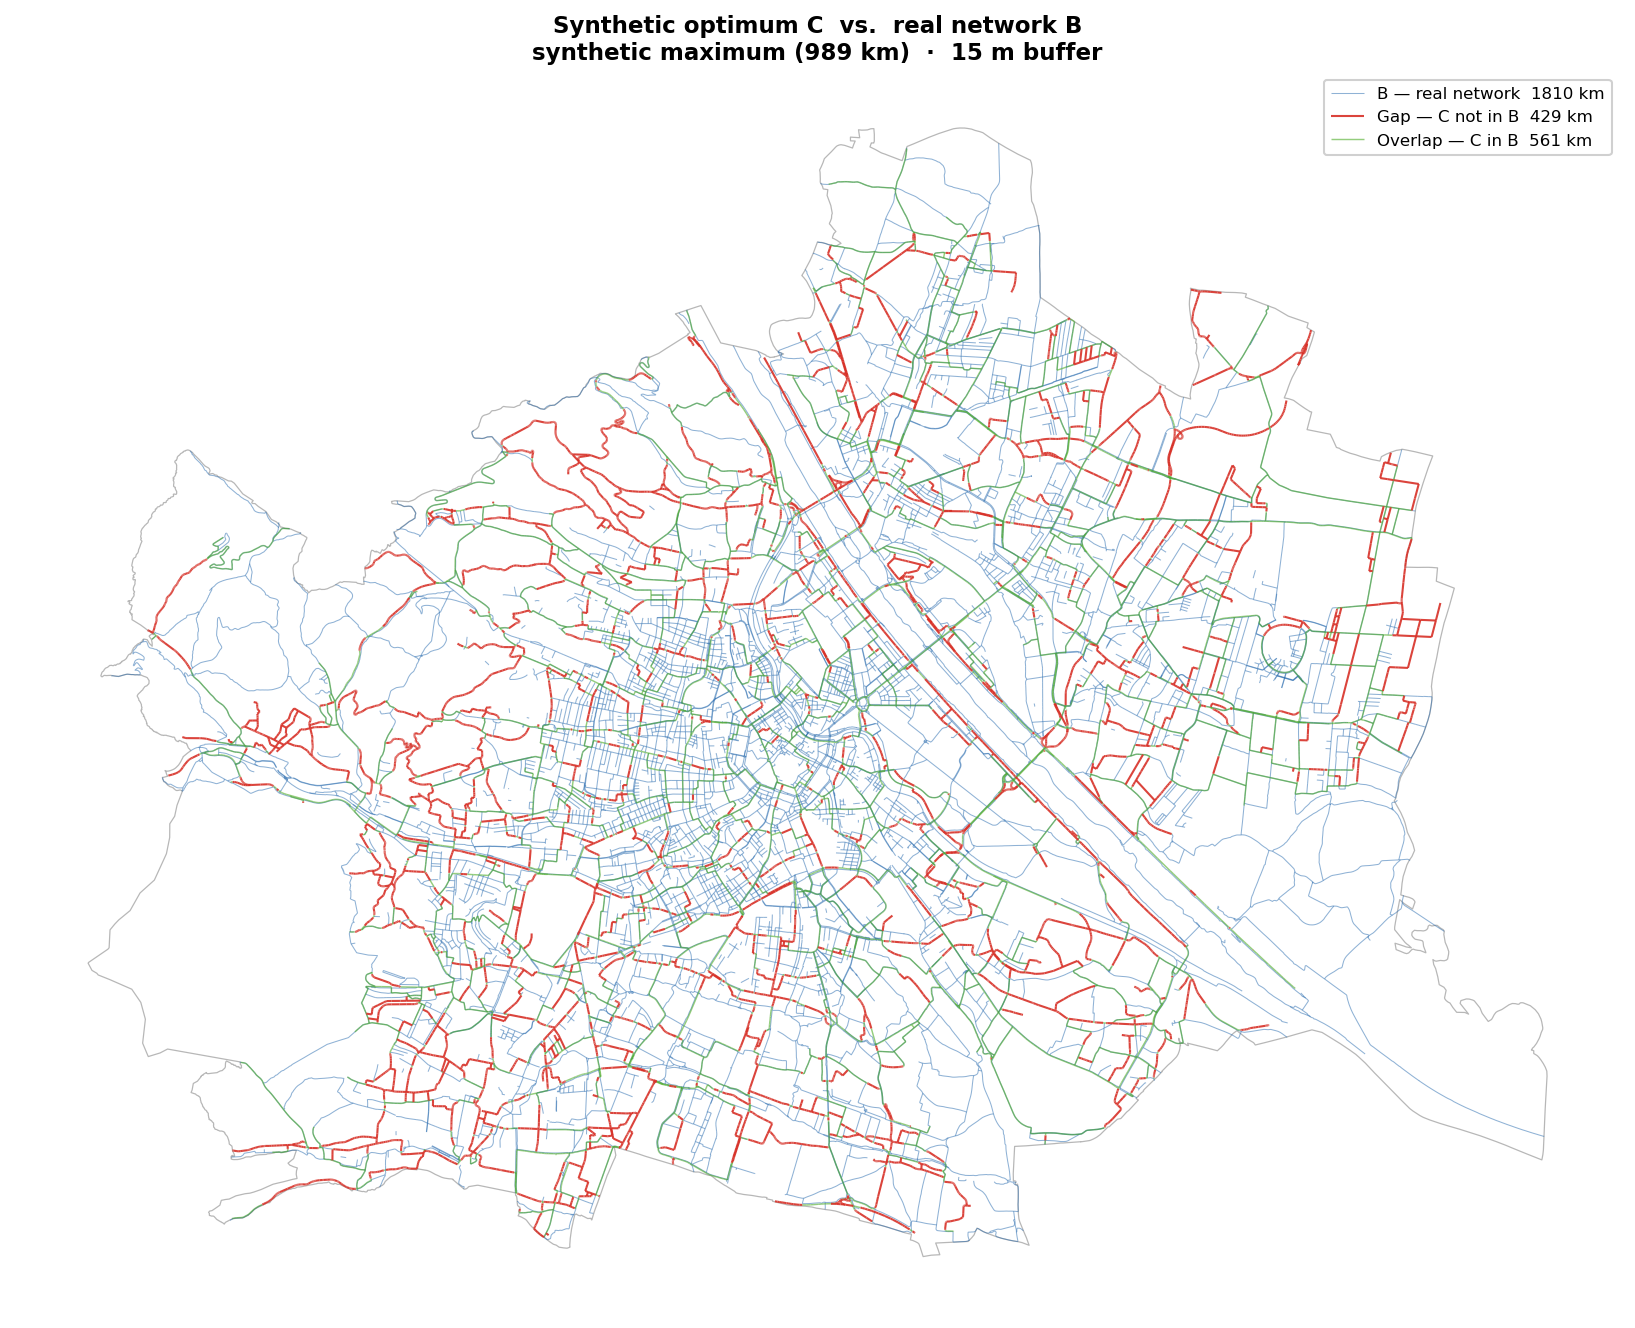
\includegraphics[width=0.78\linewidth]{vienna_overlap_gap.png}
\caption{Synthetic optimum (C) overlaid on the real network (B). Green marks the 561\,km
already built, red the 429\,km of missing strategic links, and grey the real network. The
core is dense and mostly green, while the red gaps concentrate towards the periphery.}
\label{fig:overlap}
\end{figure}

\subsection{Safe infrastructure (A): reach versus connectivity}
\label{sec:safe}

Isolating the physically protected paths, network A, gives the report's sharpest result.
This is the infrastructure most cyclists consider safe. A reaches 80\,\% of Vienna's area
within 500\,m, nearly as much as the full network's 90.7\,\%, so a protected path is almost
always close by. Yet A is shattered: only 18\,\% of its 859\,km lies in one connected
component, and the rest splinters into 2{,}360 islands, against 546 for the full network
(Fig.~\ref{fig:safe}). Reach and connectivity have come completely apart.

The practical meaning is direct. A safety-conscious cyclist can find a protected path
almost anywhere but cannot ride a continuous protected route, and is repeatedly forced onto
unsafe streets to bridge the fragments. For the safe network the bottleneck is unambiguously
connectivity, not reach. Adding kilometres would barely help; joining the existing islands
is what would turn near-universal reach into a usable safe system.

\begin{figure}[t]
\centering
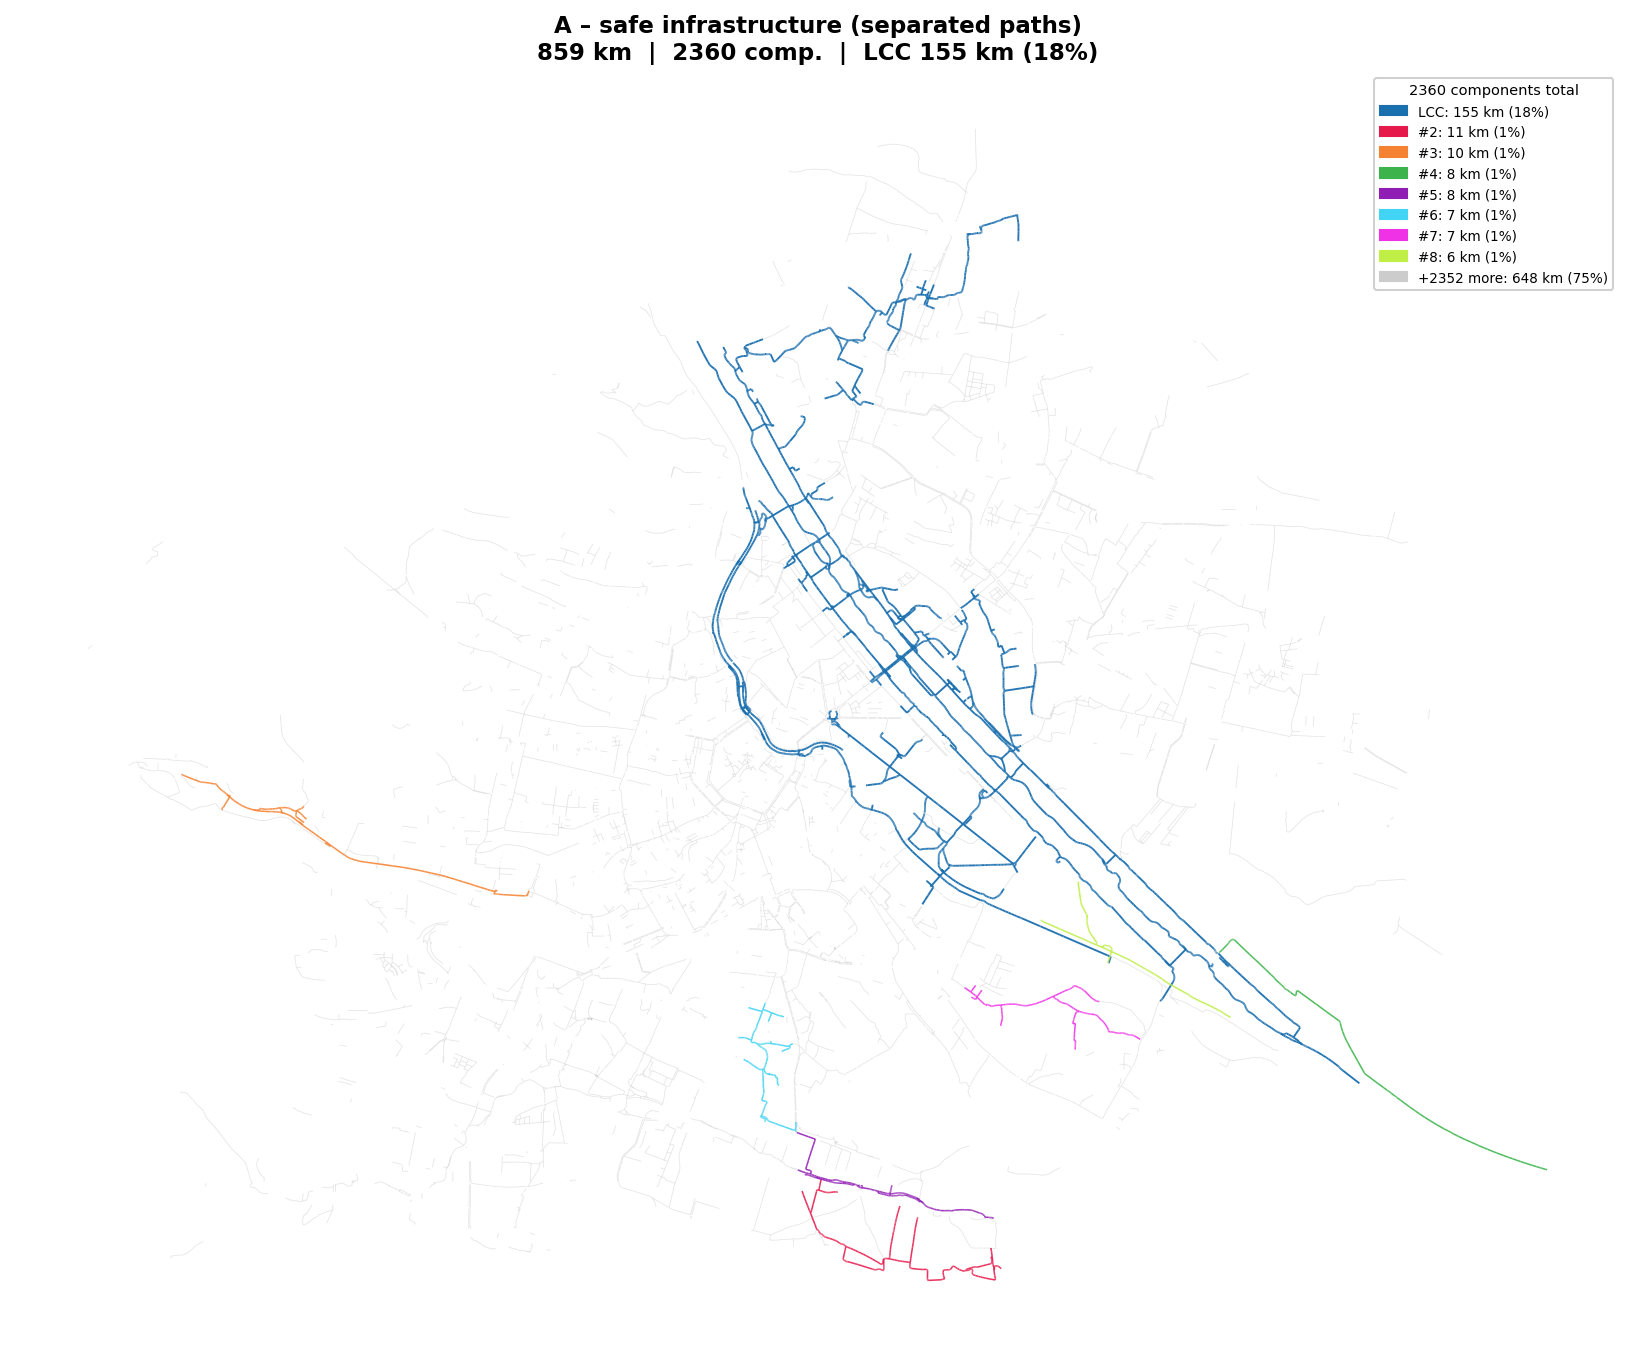
\includegraphics[width=0.74\linewidth]{vienna_safe_infra.png}
\caption{Fragmentation of the safe network (A). Dark blue marks the largest connected
component, just 155\,km or 18\,\%. Despite covering 80\,\% of the city, the protected
network is otherwise split into 2{,}360 isolated pieces.}
\label{fig:safe}
\end{figure}

\section{Vienna in a five-city context}
\label{sec:crosscity}

The second part of the results places Vienna in an international context by running the
same pipeline for four other European cities on OSM data, with the standard 1701\,m grid.
The four comparison cities were chosen to span a wide range of cycling cultures and urban
forms rather than to form a matched set: Amsterdam as a mature cycling capital, Barcelona
as a dense and compact grid, Berlin as a large polycentric metropolis, and Oslo as a
sparse, topographically constrained network. Between them they bracket Vienna on size,
density and maturity, so that whatever pattern Vienna shows can be read against a meaningful
spread. Table~\ref{tab:crosscity} reports density, directness, global efficiency and the
spatial overlap, with directness and efficiency given for both the real network (B) and the
optimum (C), so that each city can be read on its own and against its benchmark; the LCC
shares discussed below come from the same per-city results.

\subsection{Growth dynamics}

Tracing each optimum stage by stage reveals a strikingly consistent pattern across all five
cities. Every optimum collapses from many components to one and reaches almost full LCC
share within the first 20 to 30\,\% of its growth, while both directness and global
efficiency rise steeply at first and then plateau. The algorithm's structural advantage is
thus built early, by wiring up a connected backbone before later growth adds coverage. This
is exactly the regime the real networks have not completed: they have the length of a
late-stage network but the fragmentation of an early-stage one.

\subsection{Density and normalisation}

Cities differ enormously in size, with Berlin's effective area more than eight times
Barcelona's, so raw lengths are not comparable. Dividing by effective area gives network
density, reported in Table~\ref{tab:crosscity}. Real cycling density (B) varies almost
threefold, from 5.3\,km/km\textsuperscript{2} in Oslo to 15.3\,km/km\textsuperscript{2} in
Barcelona, with Vienna mid-table at 8.8. Density does not track structural quality, however:
the densest cities are not the most efficient ones, which is why the structural metrics, not
length or density, carry the argument.

\subsection{Real versus synthetic, per metric}

Reporting B and C side by side for each metric in Table~\ref{tab:crosscity} yields the
central cross-city insight: the optimum is not uniformly better than reality. Because the
real network B is much longer than the lean optimum C, the dense, well-connected real
networks of Amsterdam and Barcelona match or even exceed C on global efficiency, Amsterdam
scoring 0.688 against 0.612. Where the real network is fragmented, the optimum instead
improves efficiency dramatically, lifting Oslo from 0.102 to 0.616 and Berlin from 0.356 to
0.684. The deciding factor is connectivity rather than size: B's LCC share ranges from just
9\,\% in Oslo to 96\,\% in Amsterdam, and global efficiency follows that ordering closely.
This confirms across five cities the density-versus-structure distinction already seen for
Vienna, that more kilometres do not imply better structure.

\subsection{Per-city profiles}

Figure~\ref{fig:ccmaps} overlays each optimum on its own real network, with overlap in
green and the missing gap in red. Read together with Table~\ref{tab:crosscity}, the maps
give each city a distinct signature. The amount and location of red is the quickest visual
summary: a mostly green map means the optimum is largely already built, while long red
stretches mark where the strategic skeleton is still missing, typically towards the edges
of the city.
\begin{itemize}\setlength{\itemsep}{2pt}
\item \textbf{Amsterdam} is a dense, mature network. It has the highest overlap at 75.7\,\%
      and the smallest gap relative to its size, so its map is almost entirely green: the
      central routes already exist.
\item \textbf{Barcelona} has the densest real network, 15.3\,km/km\textsuperscript{2} in the
      smallest area, and the smallest absolute gap at 65\,km. Little is missing, and its map
      shows only short red segments.
\item \textbf{Berlin} is the largest city and has the longest optimum. That optimum scores
      highest of all five on both directness, 0.772, and efficiency, 0.684, yet the real
      network is markedly fragmented at 69\,\% LCC share and 0.356 efficiency, so the room
      for improvement is large and its map carries substantial red.
\item \textbf{Oslo} is the structural outlier. It is the sparsest at
      5.3\,km/km\textsuperscript{2}, has the lowest overlap at 31.8\,\%, and a real network
      barely connected at 9\,\% LCC share and 0.102 efficiency. Its map is the reddest of
      the five.
\item \textbf{Vienna} is balanced. It ranks second of five on the optimum's directness,
      0.730, and efficiency, 0.674, but only mid-table on density and on overlap at 62\,\%.
      The structure is sound; the real network is simply less dense and less aligned with
      the optimum than the leaders, and its map mixes green corridors with red gaps towards
      the edges.
\end{itemize}
Vienna's synthetic values here differ slightly from Table~\ref{tab:glance} because of the
coarser grid, as discussed in Sec.~\ref{sec:limits}.

\begin{table}[t]
\centering
\caption{Five-city comparison (OSM data, \(\texttt{gridl}=1701\)). B = full real network,
C = synthetic optimum; directness and global efficiency reported for both.}
\label{tab:crosscity}
\small
\begin{tabular}{lccccccc}
\toprule
& Area & B dens. & \multicolumn{2}{c}{Directness} & \multicolumn{2}{c}{Glob.\ eff.} & Overlap \\
\cmidrule(lr){4-5}\cmidrule(lr){6-7}
City & (km\textsuperscript{2}) & (km/km\textsuperscript{2}) & B & C & B & C & C in B \\
\midrule
Amsterdam & 174.5 & 12.34 & 0.630 & 0.673 & 0.688 & 0.612 & 75.7\,\% \\
Barcelona & 79.2  & 15.29 & 0.741 & 0.659 & 0.675 & 0.671 & 69.8\,\% \\
Berlin    & 664.5 & 9.39  & 0.603 & 0.772 & 0.356 & 0.684 & 75.2\,\% \\
Oslo      & 167.7 & 5.28  & 0.585 & 0.688 & 0.102 & 0.616 & 31.8\,\% \\
\textbf{Vienna} & 325.2 & 8.78 & 0.697 & 0.730 & 0.549 & 0.674 & 62.1\,\% \\
\bottomrule
\end{tabular}
\end{table}

\begin{figure}[p]
\centering
\begin{minipage}[t]{0.48\linewidth}\centering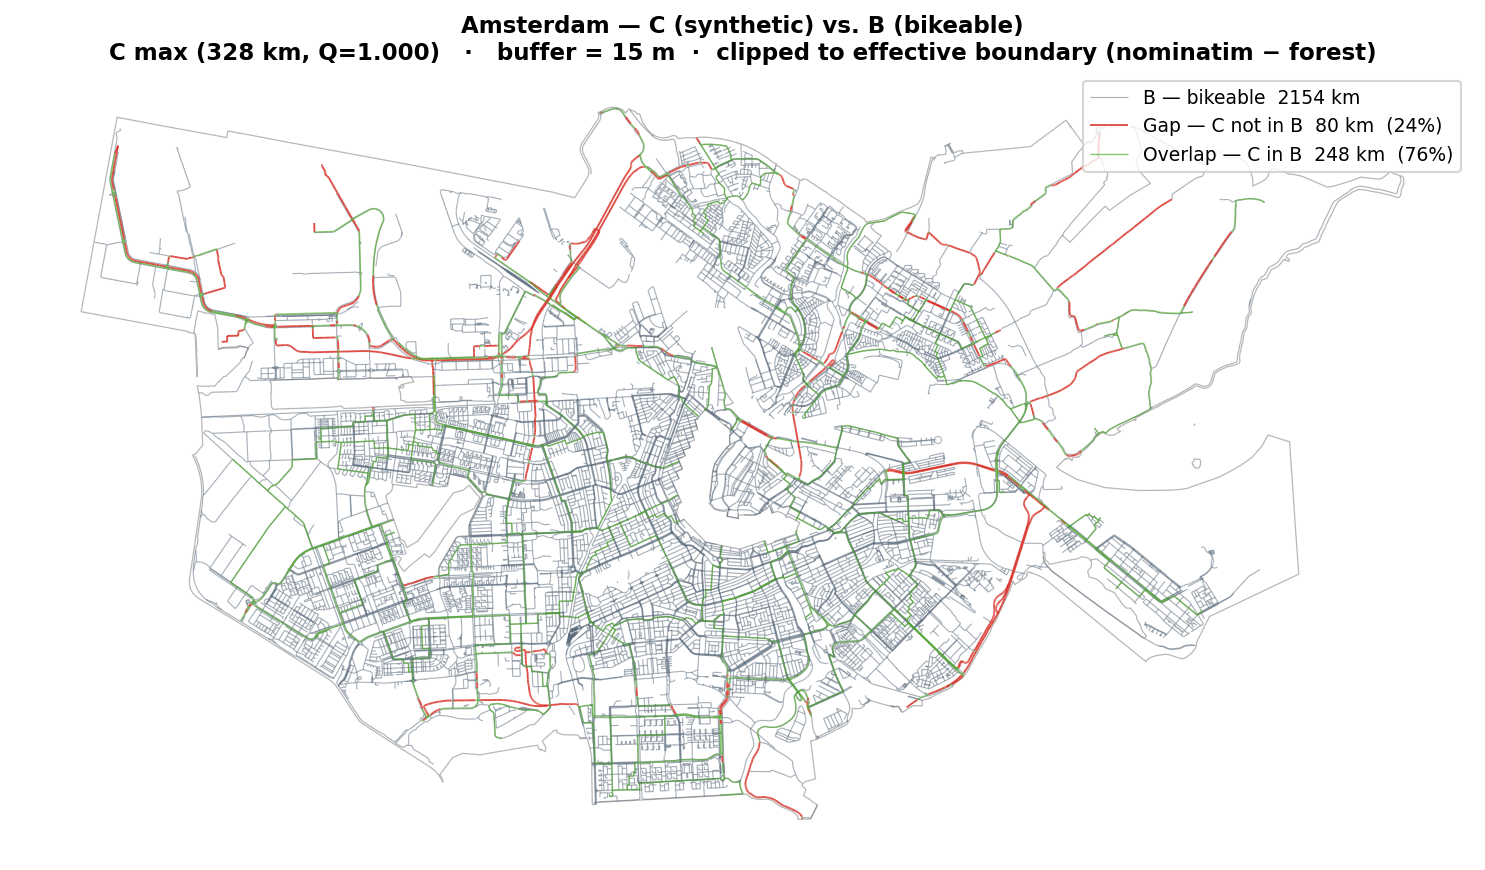
\includegraphics[width=\linewidth]{map_amsterdam.png}\end{minipage}\hfill
\begin{minipage}[t]{0.48\linewidth}\centering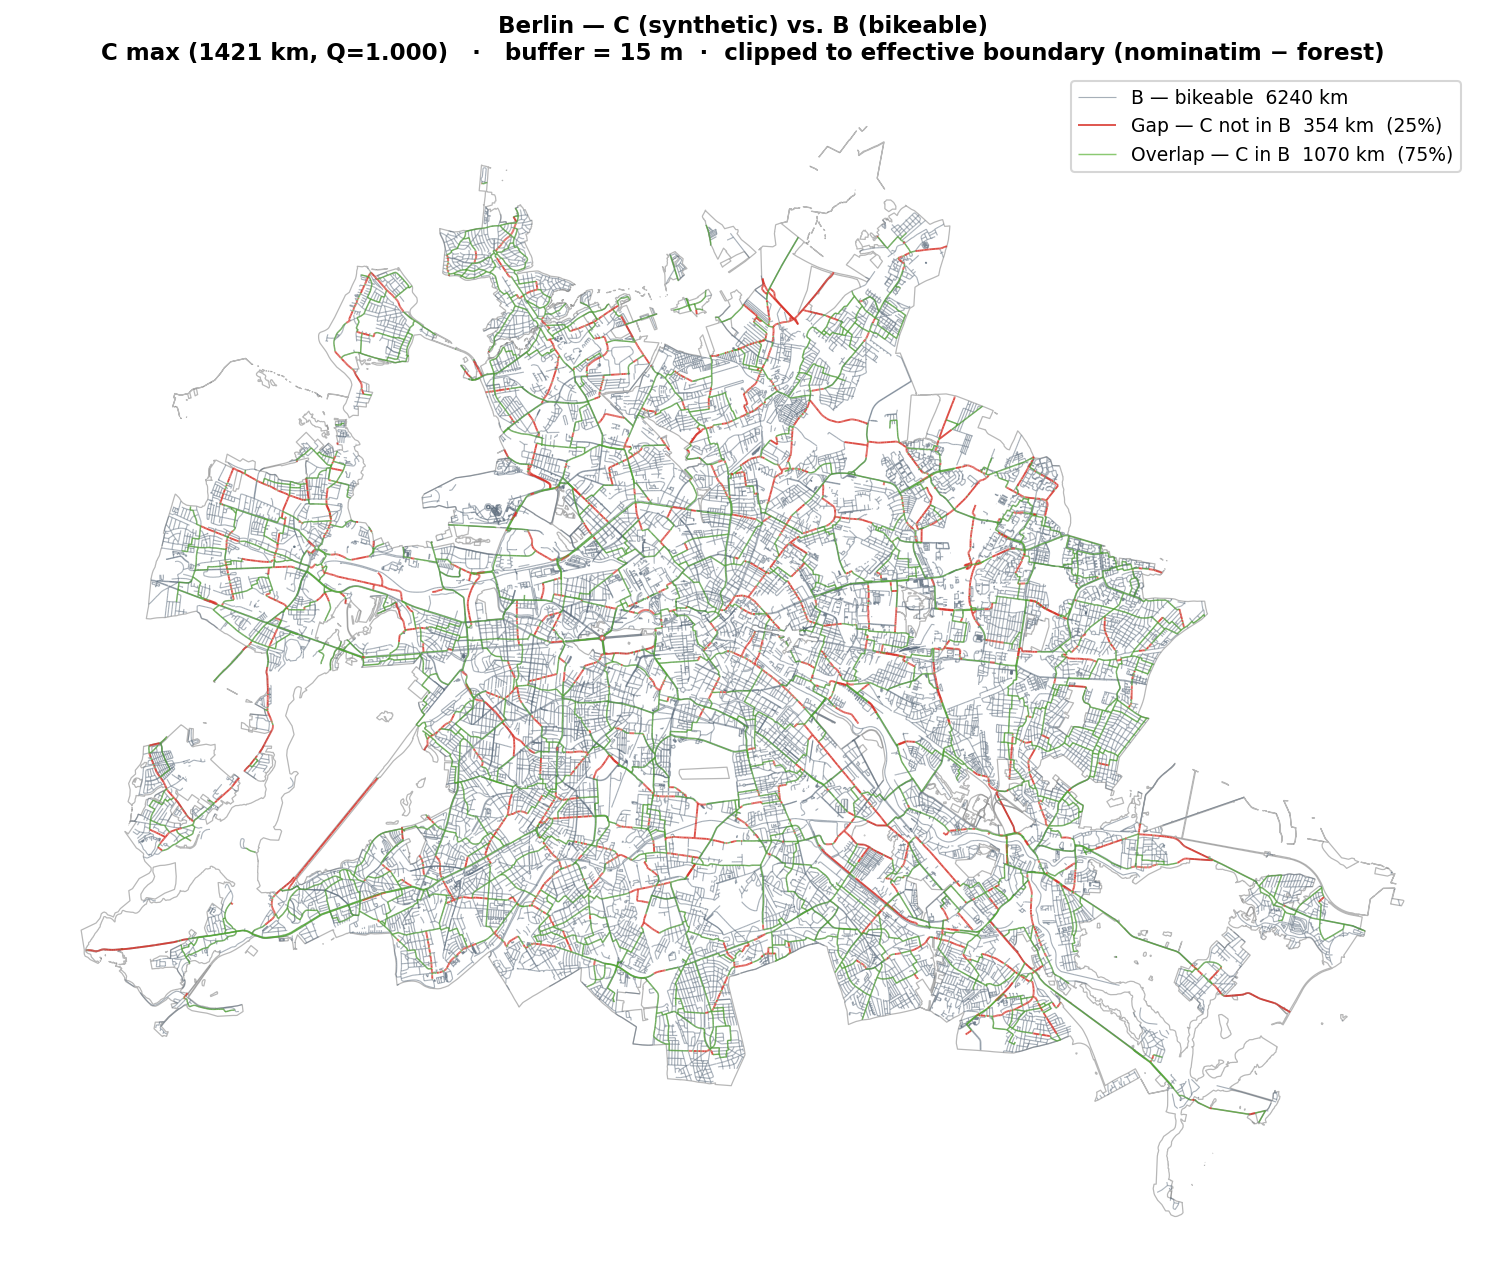
\includegraphics[width=\linewidth]{map_berlin.png}\end{minipage}

\vspace{0.6em}
\begin{minipage}[t]{0.48\linewidth}\centering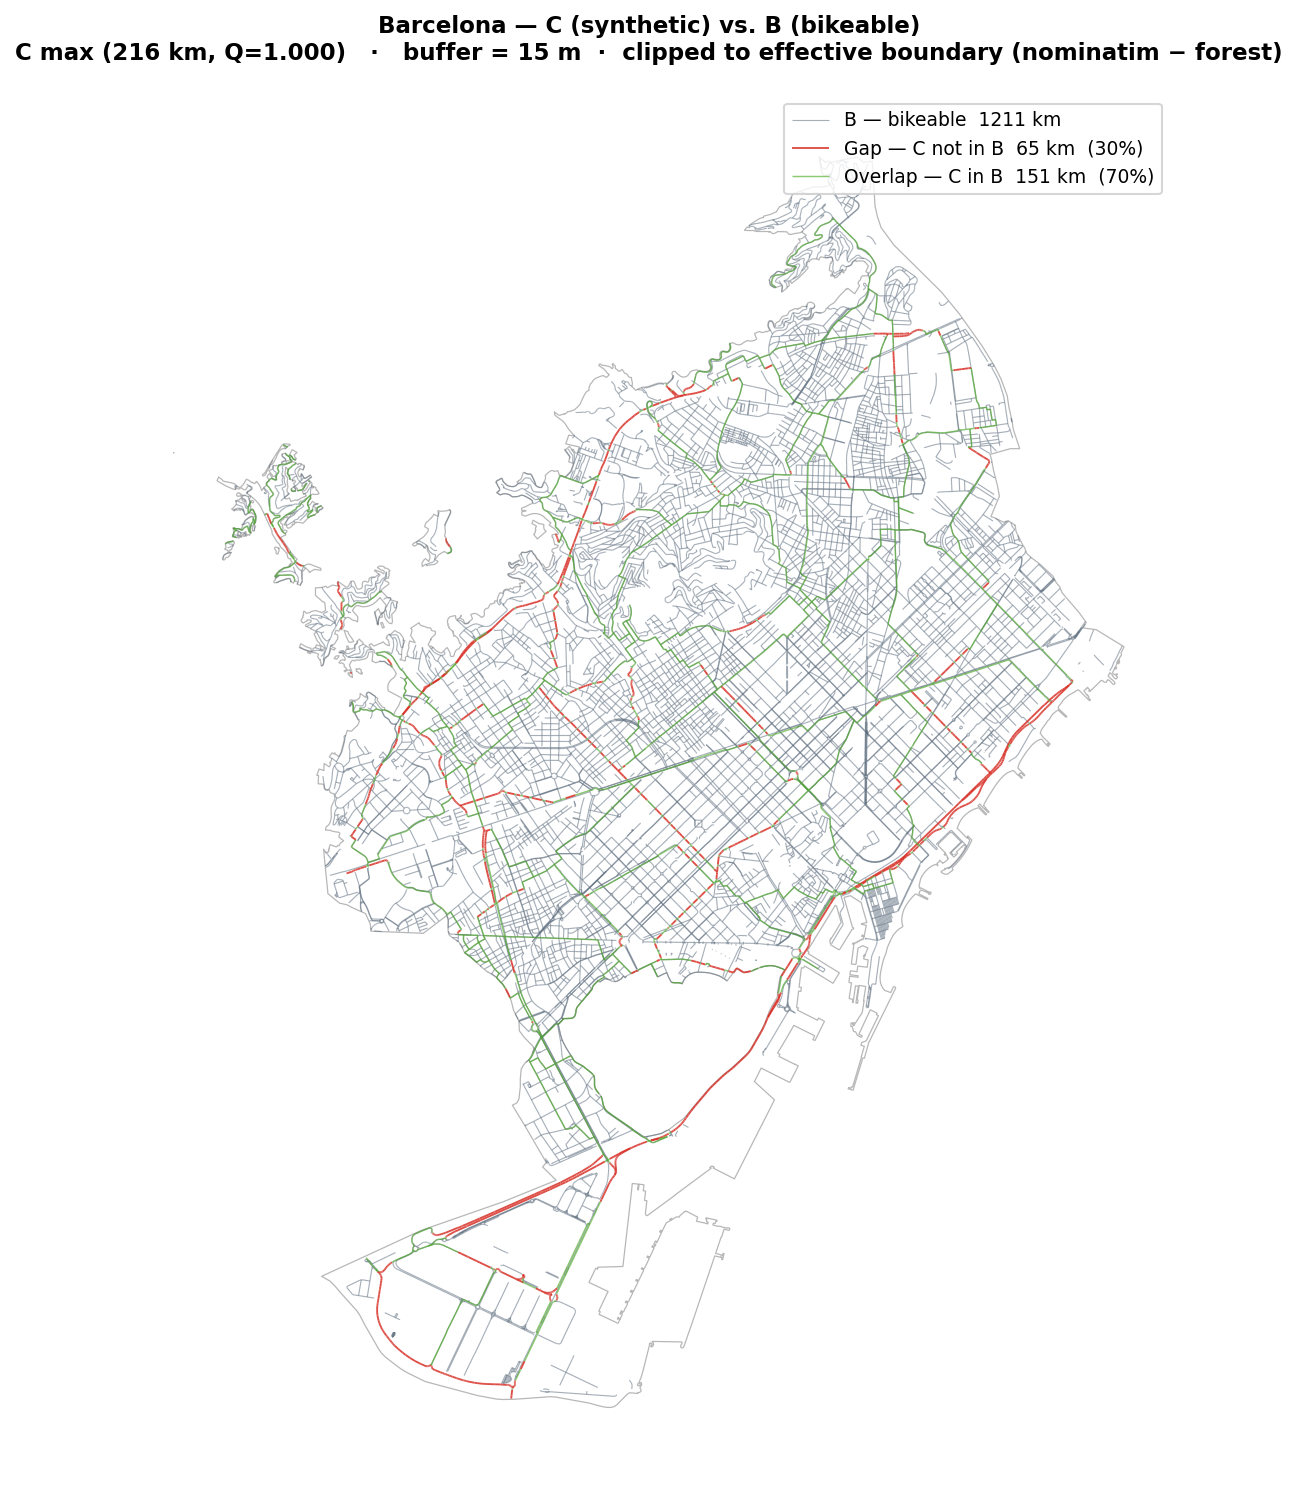
\includegraphics[width=\linewidth]{map_barcelona.png}\end{minipage}\hfill
\begin{minipage}[t]{0.48\linewidth}\centering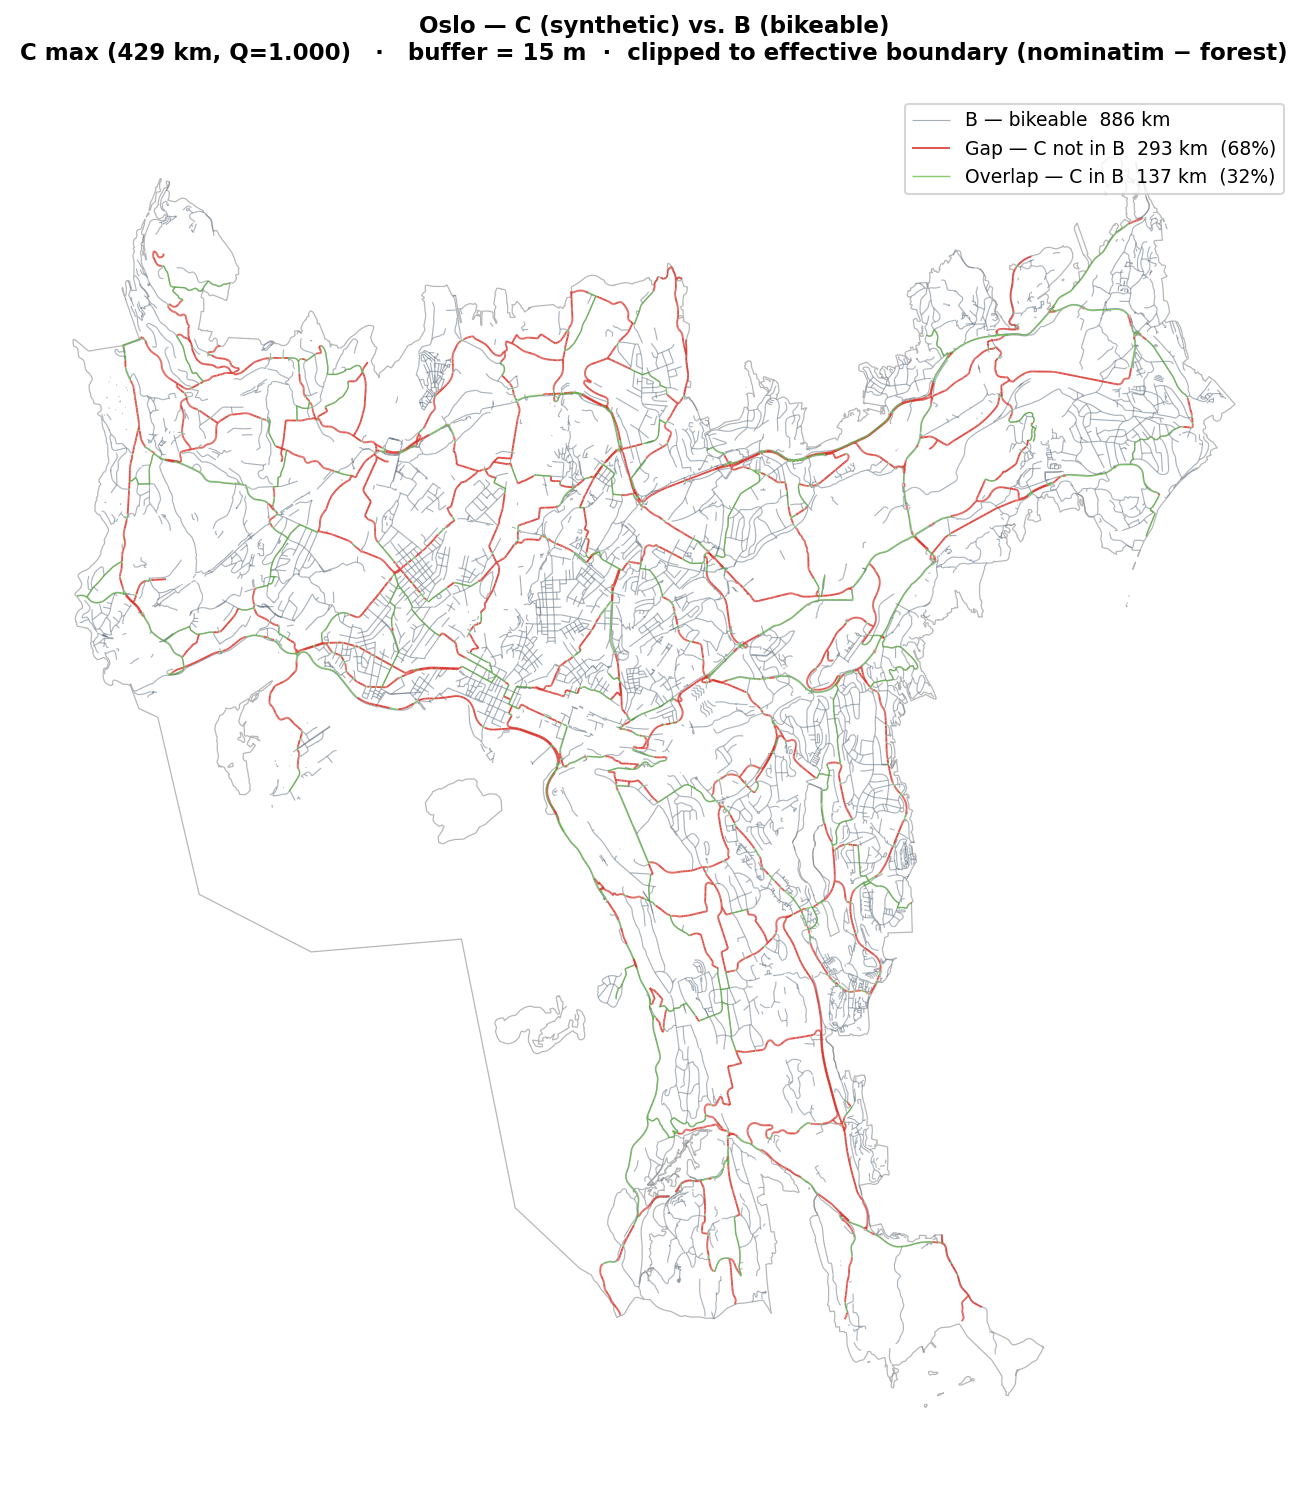
\includegraphics[width=\linewidth]{map_oslo.png}\end{minipage}

\vspace{0.6em}
\begin{minipage}[t]{0.48\linewidth}\centering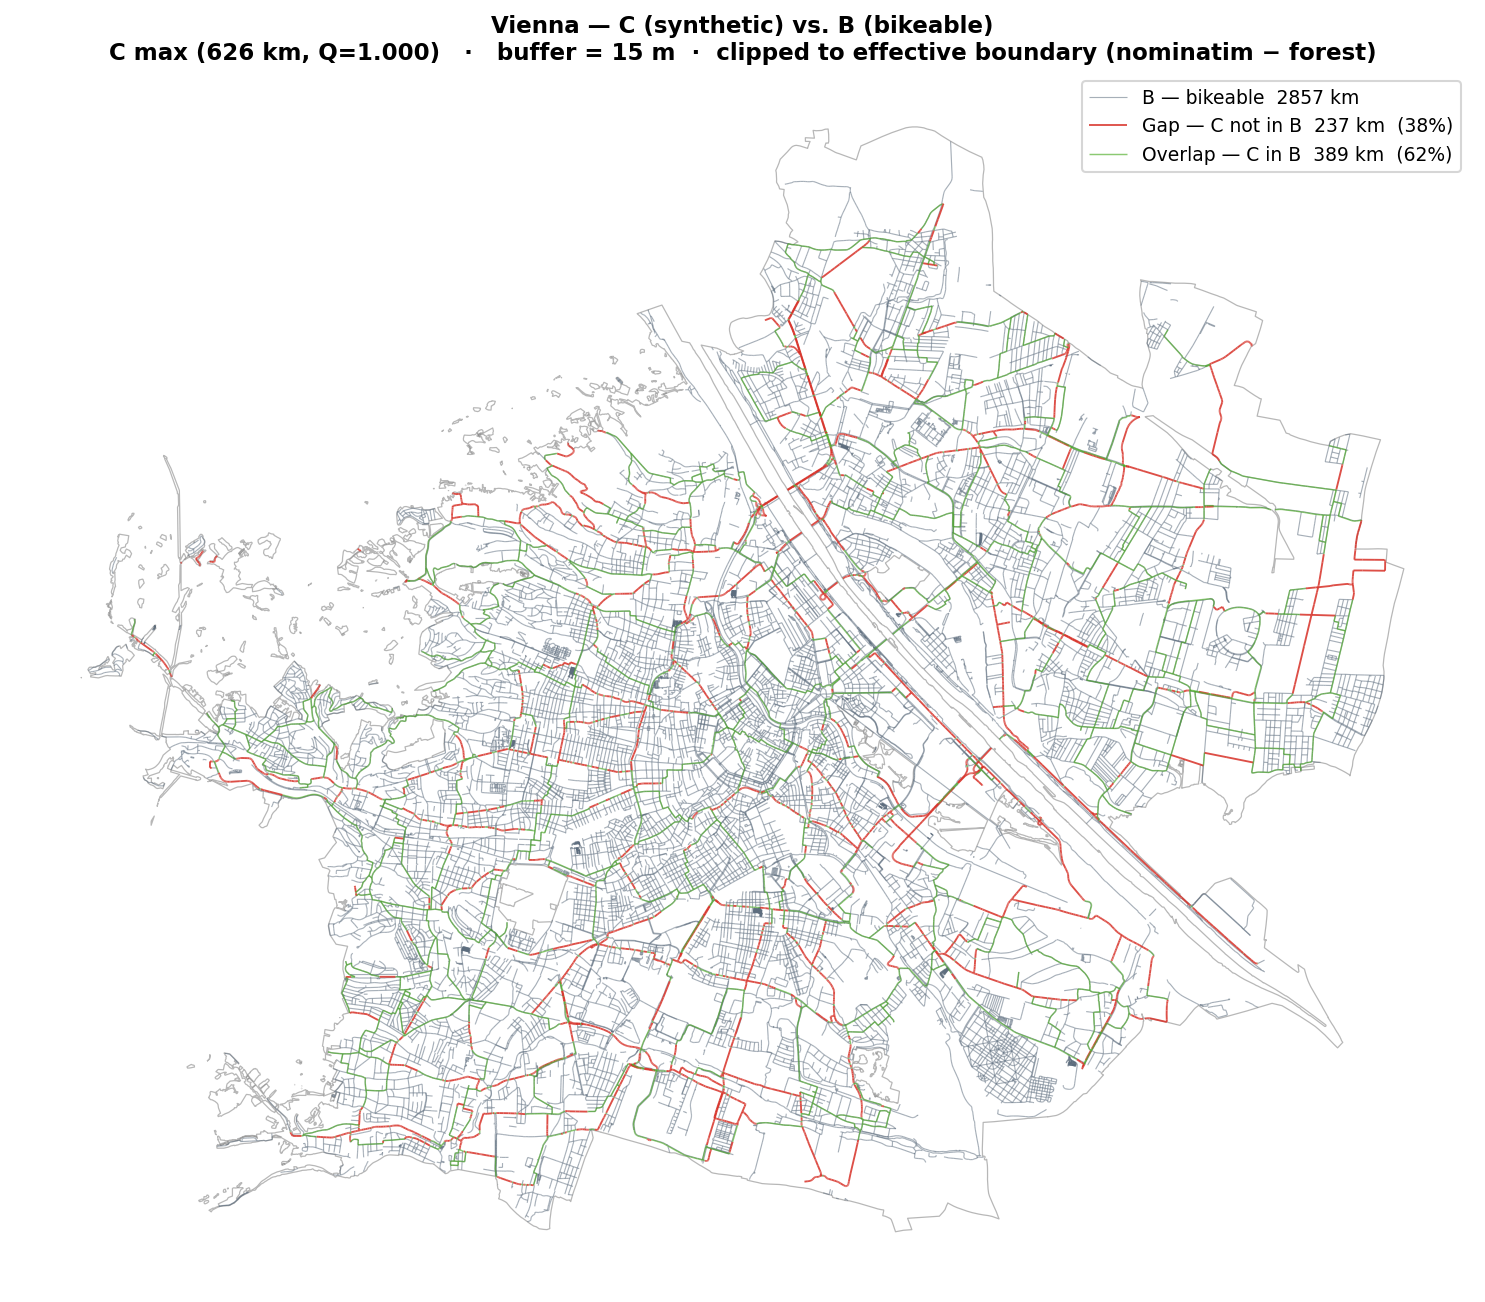
\includegraphics[width=\linewidth]{map_vienna.png}\end{minipage}
\caption{Synthetic optimum overlaid on each real network, one panel per city: green where
the optimum is already built (overlap), red where it is missing (gap), grey for the real
network. Each panel's title gives that city's overlap and gap in km. Amsterdam, Barcelona
and Berlin are largely green, while Oslo shows by far the largest red gap.}
\label{fig:ccmaps}
\end{figure}

\subsection{Safe infrastructure across cities (A versus C)}
\label{sec:safetycross}

The comparison so far has used the full rideable network B, but much of B is mixed
traffic rather than infrastructure most cyclists would consider safe. Repeating the
five-city comparison against the protected layer A, the dedicated and segregated cycle
infrastructure tagged in OpenStreetMap, with cyclist crossings snapped on as connectors,
turns the analysis into a safety question. This OSM-based A is defined differently from the
official OGD protected layer used for Vienna in Sec.~\ref{sec:safe} (a different source and
tagging, and built as a routable graph), so the two Vienna figures are not identical; the
cross-city values reported here are OSM-only for comparability.

Table~\ref{tab:safety} reports A for all five cities, and two patterns stand out. First,
the protected network is everywhere far more fragmented than the full network. Its largest
connected component holds only 8\,\% of the protected length in Oslo and 25\,\% in Berlin,
rising to 79\,\% in Amsterdam, against B's range of 9 to 96\,\% and the optimum's 100\,\%.
Protected density is likewise a fraction of rideable density, between 1.9 and
4.2\,km/km\textsuperscript{2} against B's 5.3 to 15.3. The safe layer is both sparser and
more broken than the network it sits inside.

Second, and most telling for safety, only a small share of the optimum already runs on
protected infrastructure: 51.4\,\% in Amsterdam falling to 14.8\,\% in Oslo, with Vienna at
19.9\,\%. The complementary gap, from 48.6\,\% to 85.2\,\% of the optimum, marks strategic
routes that today have no protected path and would be ridden in mixed traffic. This gap is a
sharper statement than the overlap with B in Table~\ref{tab:crosscity}: where B overlap asks
how much of the optimum is already rideable, A overlap asks how much is already safe, and the
two diverge widely. Vienna's optimum is 62\,\% rideable but only 20\,\% protected, and
Berlin's is 75\,\% rideable but 33\,\% protected. For every city the protected backlog is
the larger of the two, so the priority for safe cycling is less about adding length than
about upgrading and connecting the protected layer along the routes the optimum identifies.

This last point makes the optimum a concrete connectivity plan rather than only a yardstick.
Treating the gap edges as if built as protected infrastructure and adding them back to A
reconnects its islands: the protected LCC share rises from 25 to 78\,\% in Berlin, 8 to
42\,\% in Oslo, 60 to 88\,\% in Vienna, 79 to 90\,\% in Amsterdam and 79 to 91\,\% in
Barcelona (last column of Table~\ref{tab:safety}). The most fragmented networks gain the
most, which is the sharpest link back to the synthetic network: C does not merely measure
the safety gap, it identifies the specific strategic links whose construction would join the
disconnected protected islands into one usable whole. By contrast, the cyclist crossings
already folded into A move its connectivity only marginally (at most a fraction of a
percentage point of LCC share), because they bridge points that already meet at junctions
rather than the long unprotected stretches between islands; the gap links are what close
those stretches.

\begin{table}[t]
\centering
\caption{Five-city safety comparison (OSM data, \(\texttt{gridl}=1701\)). A = protected
network (biketrack, including snapped cyclist crossings); C = synthetic optimum. Overlap is
the share of C already running on protected infrastructure; the gap is its complement. The
\emph{A+gap} column gives A's LCC share if the gap links were built as protected
(island-bridging analysis).}
\label{tab:safety}
\small
\begin{tabular}{lcccccc}
\toprule
City & A dens. & A direct. & A glob.\ eff. & A LCC & A+gap & Overlap \\
 & (km/km\textsuperscript{2}) & (LCC) & & share & LCC & C in A \\
\midrule
Amsterdam & 4.20 & 0.737 & 0.420 & 79\,\% & 90\,\% & 51.4\,\% \\
Barcelona & 3.04 & 0.792 & 0.510 & 79\,\% & 91\,\% & 22.0\,\% \\
Berlin    & 2.10 & 0.608 & 0.169 & 25\,\% & 78\,\% & 32.6\,\% \\
Oslo      & 1.91 & 0.649 & 0.117 & 8\,\%  & 42\,\% & 14.8\,\% \\
\textbf{Vienna} & 2.07 & 0.608 & 0.351 & 60\,\% & 88\,\% & 19.9\,\% \\
\bottomrule
\end{tabular}
\end{table}

\begin{figure}[p]
\centering
\begin{minipage}[t]{0.48\linewidth}\centering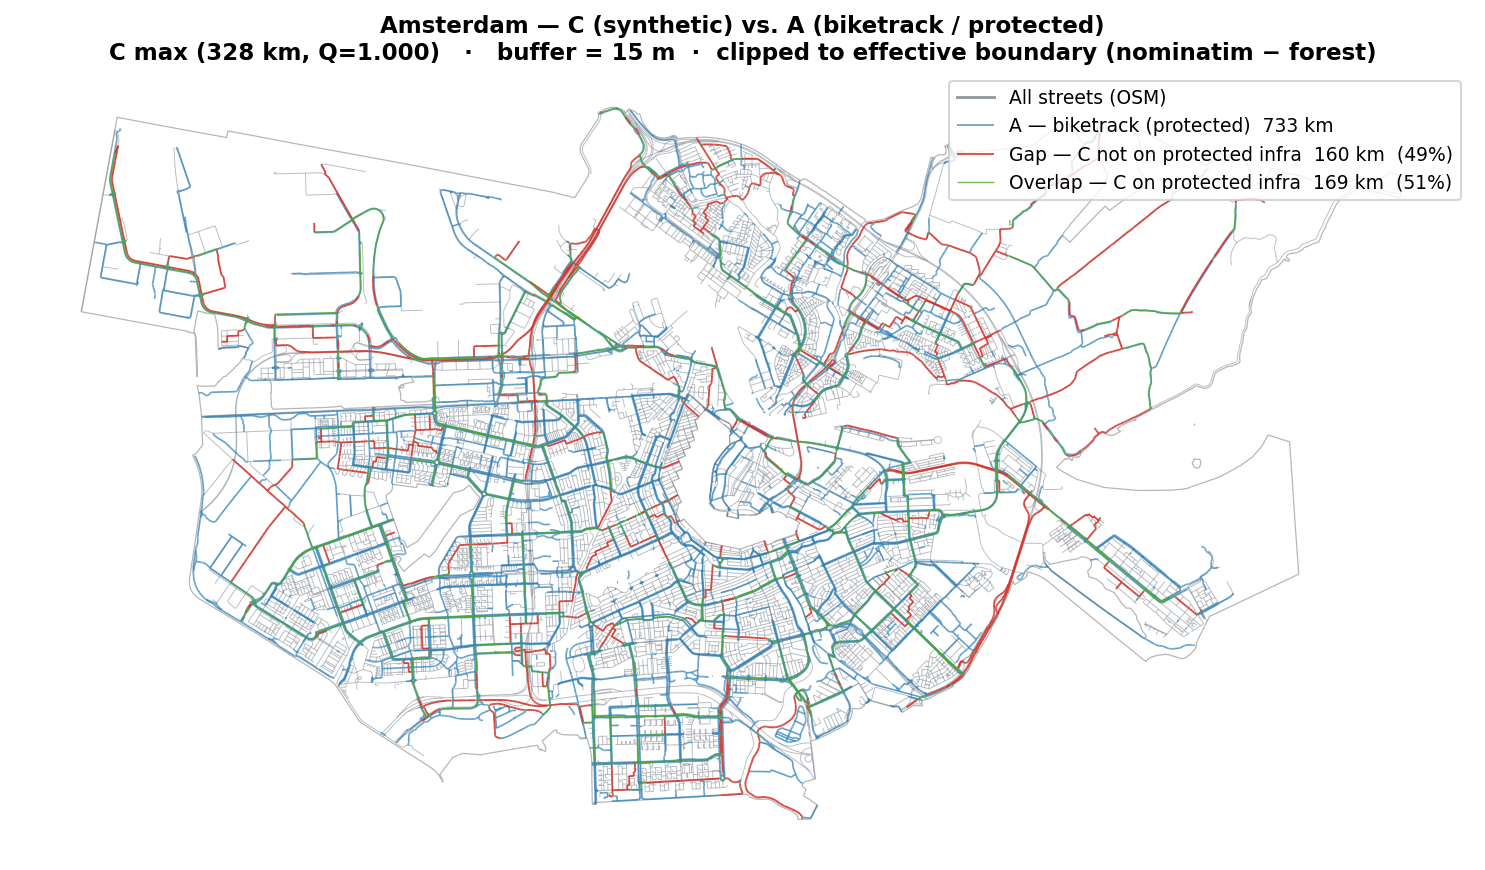
\includegraphics[width=\linewidth]{map_amsterdam_safety.png}\end{minipage}\hfill
\begin{minipage}[t]{0.48\linewidth}\centering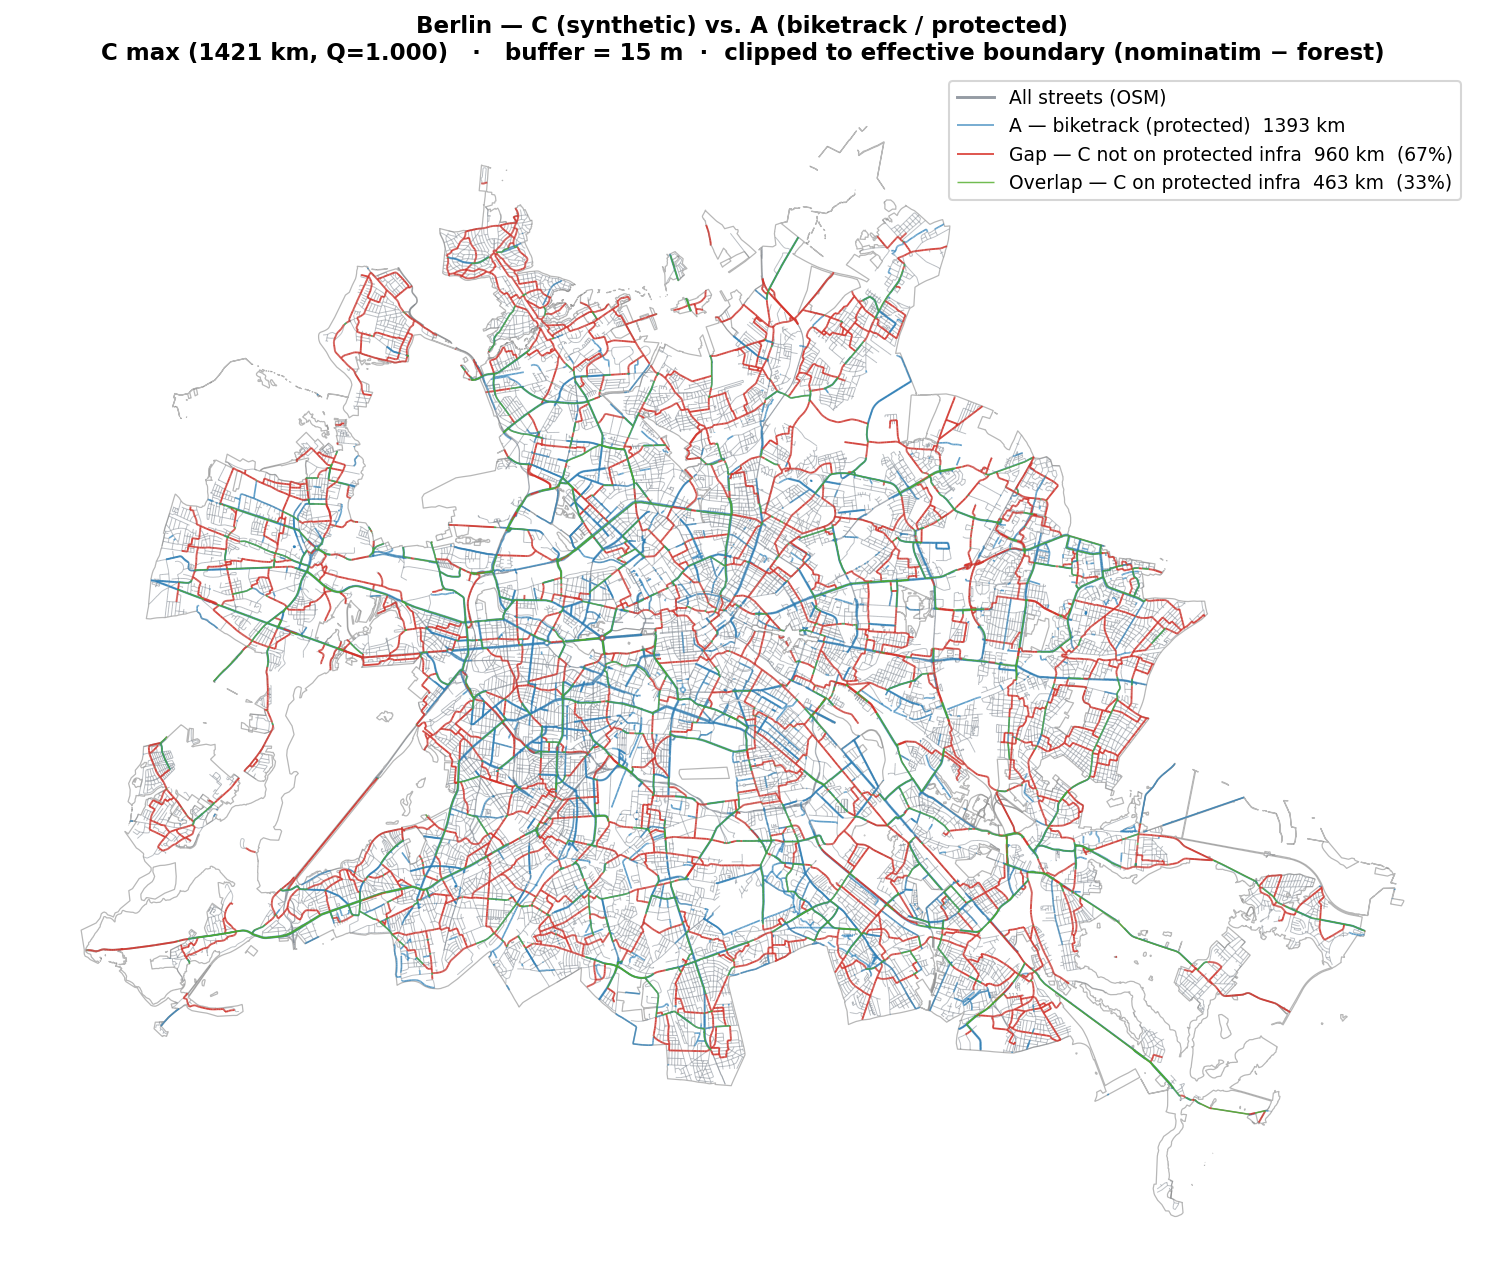
\includegraphics[width=\linewidth]{map_berlin_safety.png}\end{minipage}

\vspace{0.6em}
\begin{minipage}[t]{0.48\linewidth}\centering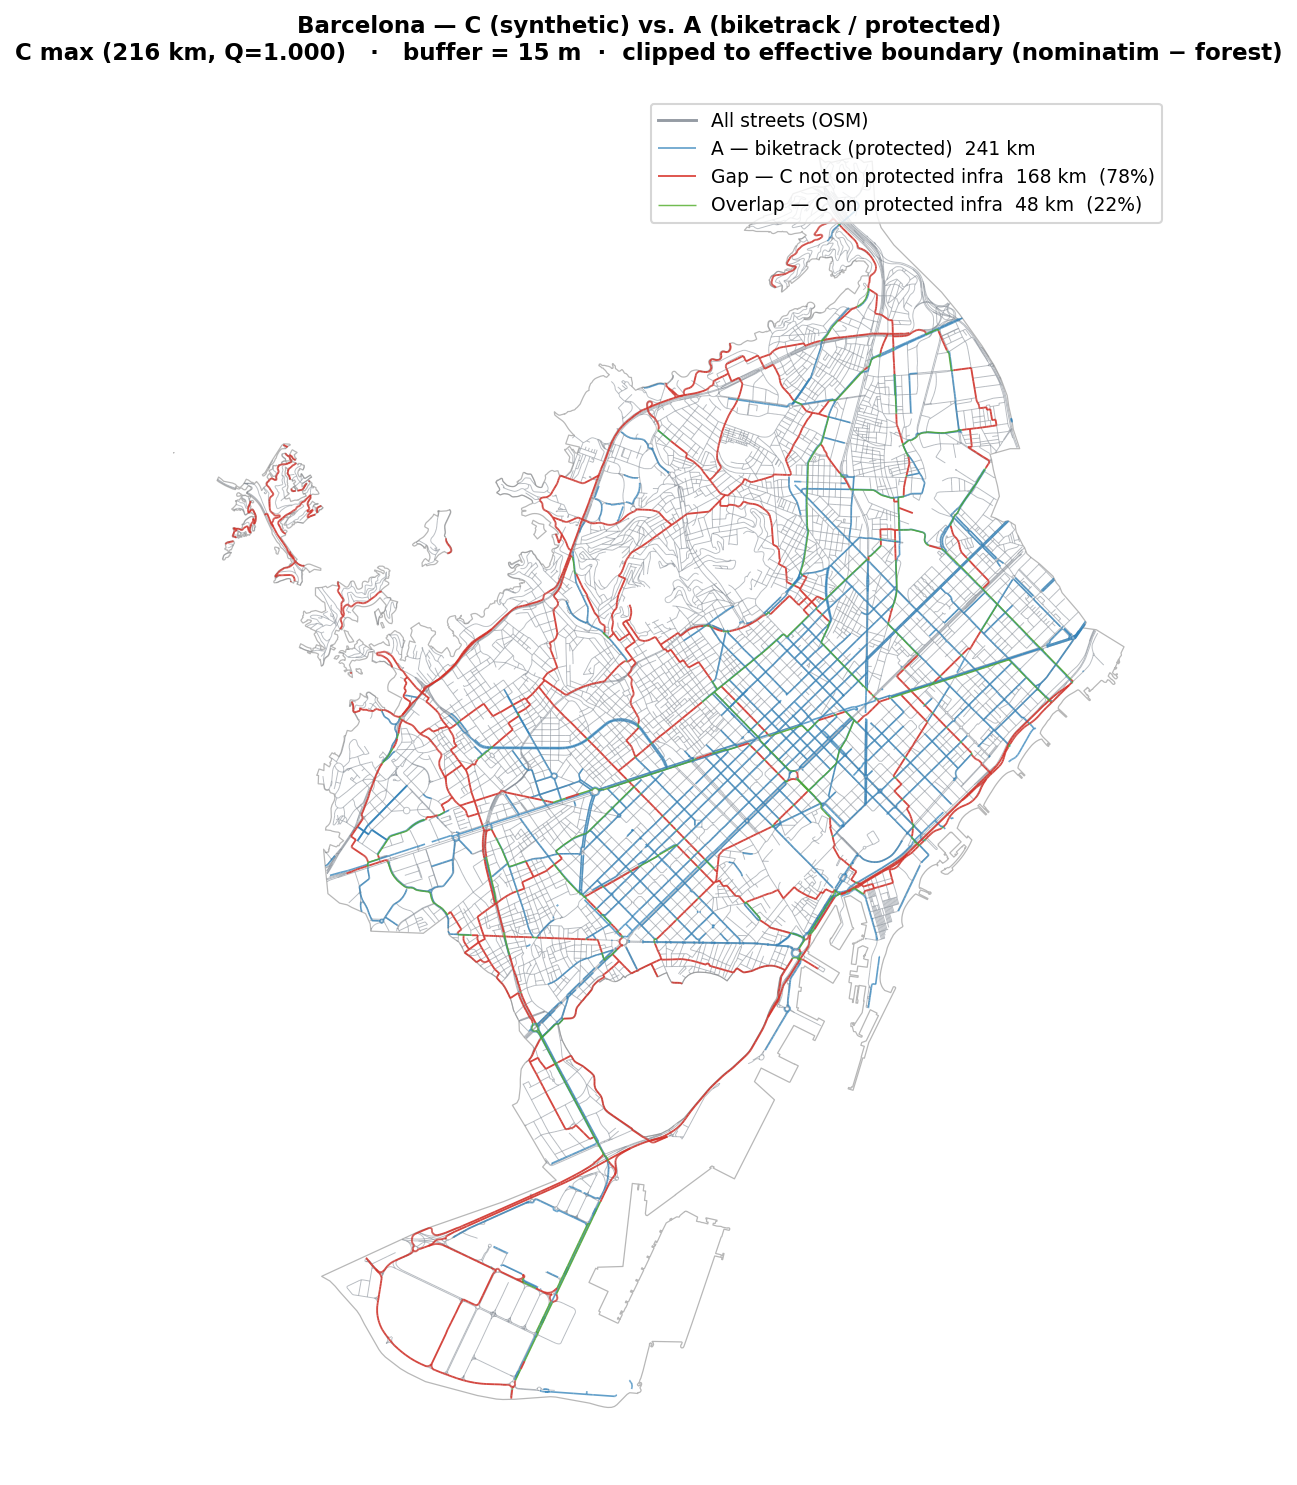
\includegraphics[width=\linewidth]{map_barcelona_safety.png}\end{minipage}\hfill
\begin{minipage}[t]{0.48\linewidth}\centering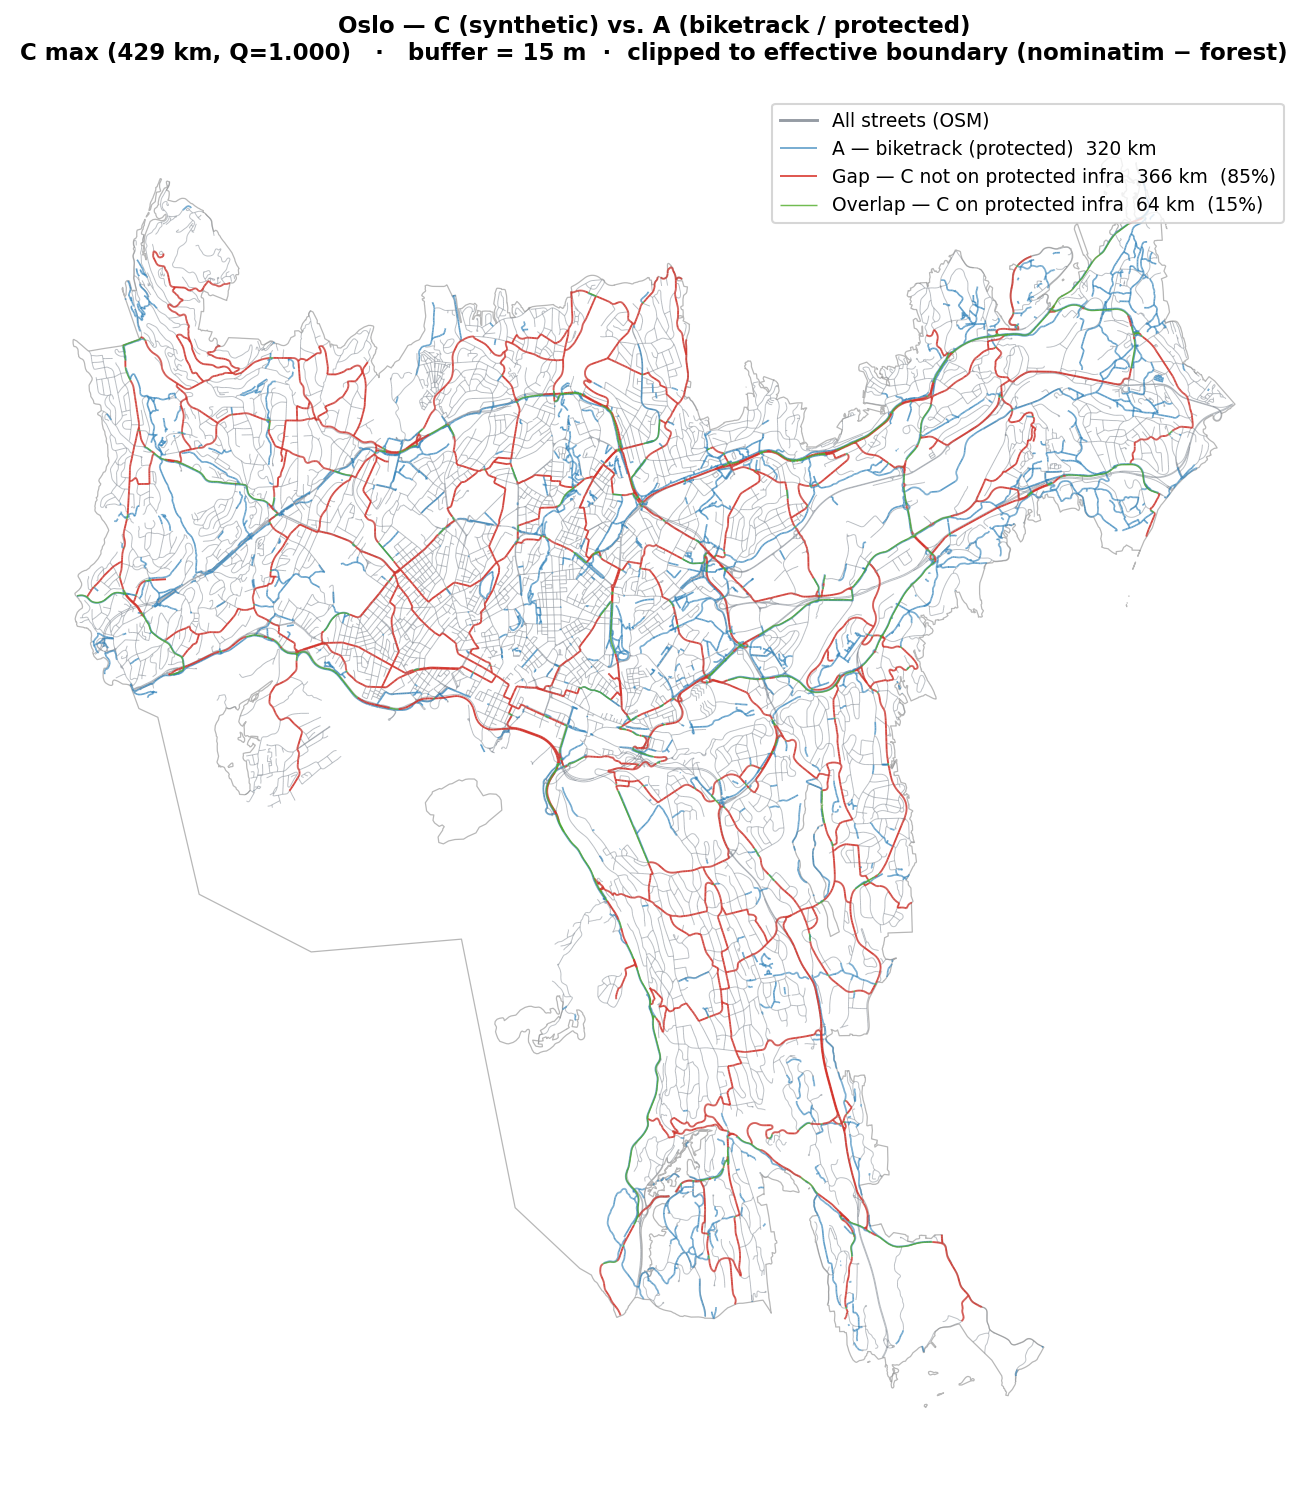
\includegraphics[width=\linewidth]{map_oslo_safety.png}\end{minipage}

\vspace{0.6em}
\begin{minipage}[t]{0.48\linewidth}\centering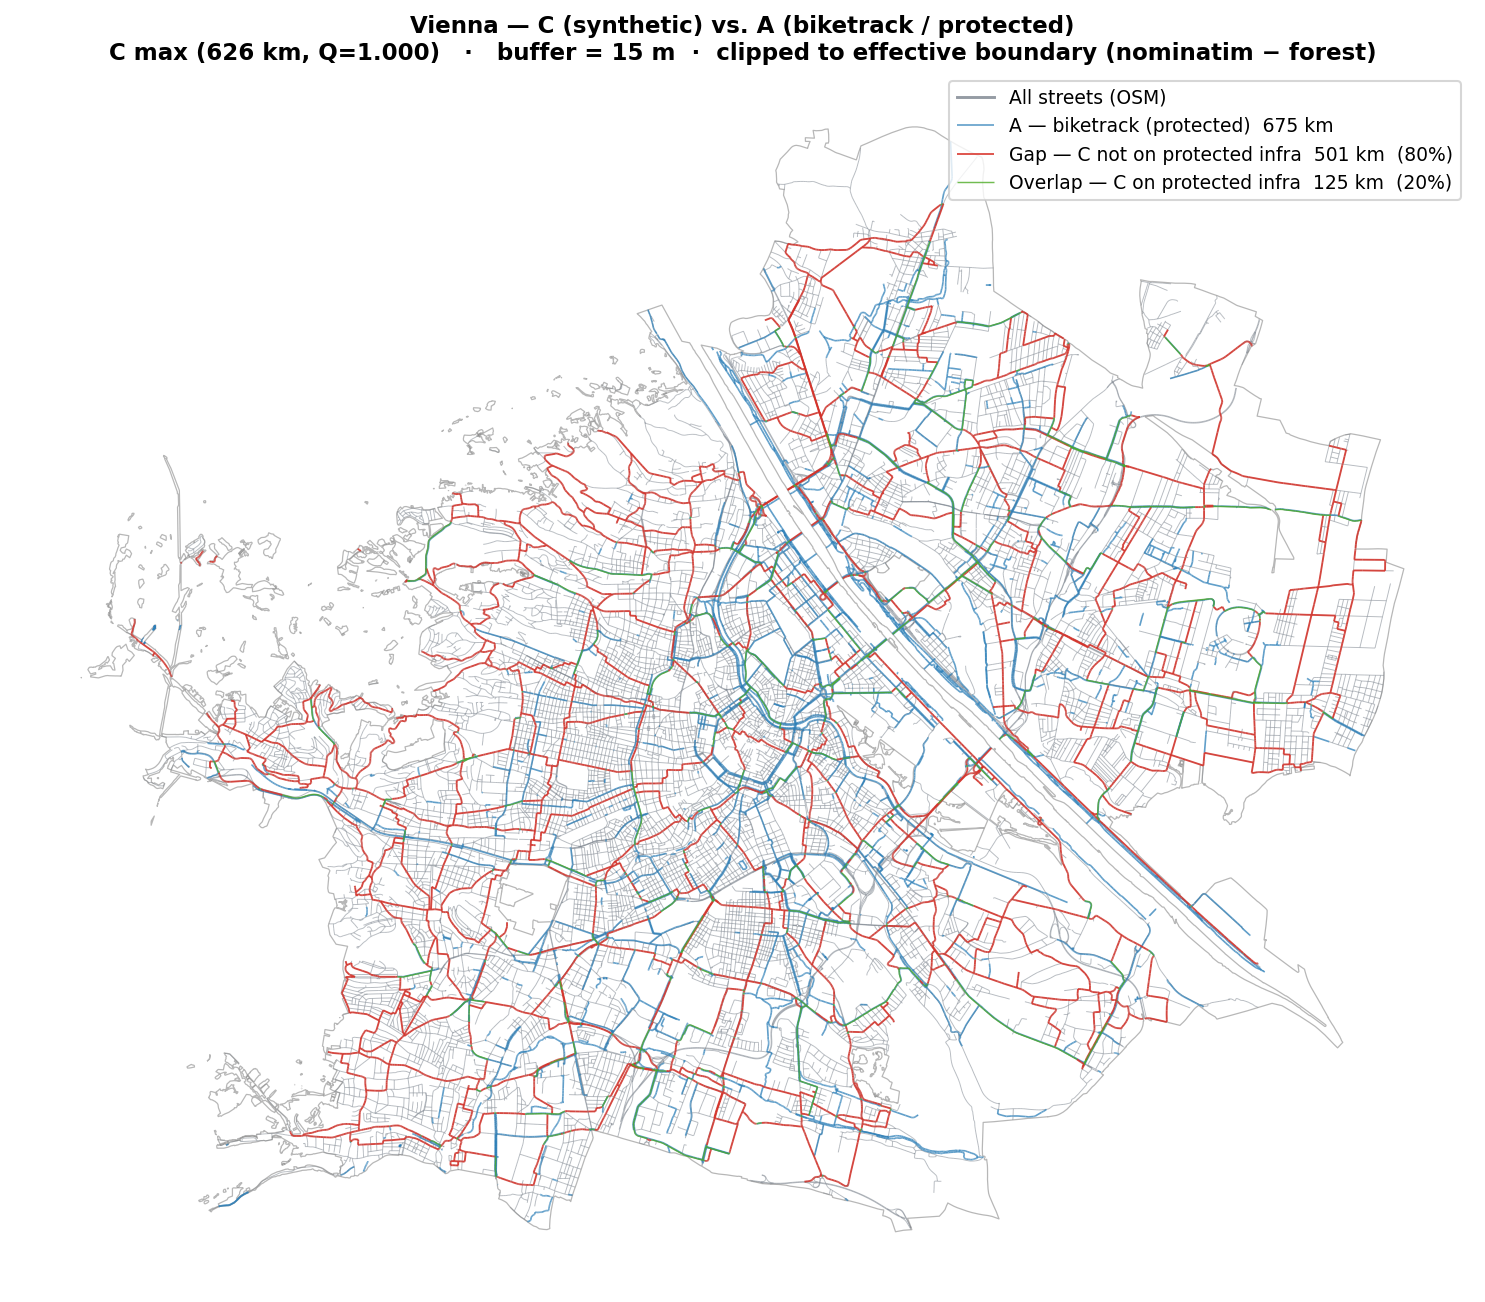
\includegraphics[width=\linewidth]{map_vienna_safety.png}\end{minipage}
\caption{Synthetic optimum overlaid on each city's protected network A, one panel per city:
blue is the protected infrastructure, green where the optimum already runs on it (overlap),
and red where it does not (unprotected gap). In contrast to the largely green B maps of
Fig.~\ref{fig:ccmaps}, red dominates every panel, the visual signature of the
protected-infrastructure backlog.}
\label{fig:safetymaps}
\end{figure}

\section{Discussion}

\paragraph{Answering the research question.} Vienna's real network is good in reach but
weaker in connection. It covers the city better than the optimum, 90.7\,\% against
89.3\,\%, and is fairly direct within its core, yet it is 14.6\,\% less globally efficient
because it is fragmented, most severely in its safe layer at 18\,\% connected. This
combination of excellent spatial distribution with sub-optimal connection is consistent
with growth that was opportunistic rather than network-planned, the third sub-question:
infrastructure was added wherever locally feasible, producing broad coverage without a
coherent connected backbone. This remains an interpretation rather than a proof, since a
direct test would require the network's growth history over time, which snapshot data
cannot provide.

\paragraph{Planning implications.} The actionable levers are topological, not metric. The
first is to connect existing fragments, above all in the safe network, where joining the
2{,}360 protected islands would convert near-universal reach into a usable connected system.
The second is to build the strategic gap links the optimum prioritises, which sit mainly in
the outer districts and offer the largest efficiency gain per kilometre, answering
sub-questions (ii) and (iv). Both are about how the network joins up rather than how long it
is, and Vienna already has more kilometres than the optimum. The five-city safety comparison
(Sec.~\ref{sec:safetycross}) shows this lever is not particular to Vienna: treating the
optimum's gap as protected infrastructure lifts the protected connected share from 25 to
78\,\% in Berlin, 8 to 42\,\% in Oslo and 60 to 88\,\% in Vienna, with the most fragmented
networks gaining the most, whereas the cyclist crossings already present barely move it.
Connecting the right strategic links, not adding kilometres, is the lever for safe cycling
across all five cities.

\paragraph{Methodological takeaway.} Treating a cycling network as a graph and a set of
reproducible structural indicators makes ``quality'' measurable and comparable, and exposes
distinctions that a length or coverage map cannot. The two most important are that reach and
connectivity can diverge sharply, as in the safe network, and that density and structural
efficiency are not the same thing, as the cross-city comparison shows.

\section{Limitations}
\label{sec:limits}

The Vienna and cross-city analyses use different data sources, OGD against OSM, and the
Vienna deep dive uses a finer 600\,m grid than the cross-city run at 1701\,m. Their absolute
lengths and Vienna's synthetic figures therefore differ between Tables~\ref{tab:glance}
and~\ref{tab:crosscity}, even though the structural conclusions agree. The synthetic optimum
is thus a representative target rather than a unique one, since a different grid yields a
longer or shorter skeleton (Fig.~\ref{fig:gridl}). Directness and global efficiency are estimated from a random
sample of nodes and so carry a small sampling variance of a few tenths of a percent. The
overlap and gap classification reflects the algorithm's betweenness-based priorities and a
fixed 15\,m buffer, not an absolute planning truth. Both networks are also single snapshots:
the real network is actively being extended, including a recent municipal programme that
explicitly targets gaps in the main network \citep{wienradprogramm}, so the 429\,km gap
reported here is a moving target rather than a fixed deficit. Finally, without the network's
growth history over time, the question of planned against opportunistic development, the
third sub-question, can be answered only from the present structure rather than directly.

\section{Conclusion}

Measured against a grown optimum, Vienna's bicycle network answers the opening question
clearly: it is excellent in reach but weak in connection, and the way it is put together
looks shaped by opportunity rather than by a network logic. It covers the city as well as
the optimum, yet it is measurably less efficient because it is fragmented, most starkly in
the safe, protected layer, which reaches 80\,\% of the city but holds only 18\,\% of its
length in one connected piece across 2{,}360 fragments. The largest structural gaps, a
focused 429\,km or 43\,\% of the optimal skeleton, sit mainly in the outer districts rather
than in the well-covered core. Internationally Vienna is solid but mid-pack. The evidence
therefore points to a clear, low-regret strategy: prioritise connecting the network, by
joining the islands of safe infrastructure and adding the few strategic links the optimum
identifies, over simply extending it. This is what the title intends by structure over
length: Vienna already has more kilometres than the optimum, and what it lacks is the way
they join up. Beyond Vienna, the contribution is a transparent, reproducible pipeline that
turns raw cycling geodata into comparable structural diagnostics, applicable to any city.

\bibliographystyle{plainnat}
\renewcommand{\refname}{References}
\bibliography{references}
\nocite{*}

\end{document}
